\chapter{大脑老化} \label{chap:chap64}

1900年美国的平均寿命约为50岁。
到 2015 年,男性约为 77 岁,女性约为 82 岁(图 \ref{fig:64_1})。
其他 30 个国家的平均水平更高。 这些增加主要是由于婴儿死亡率的降低、疫苗和抗生素的开发、更好的营养、改进的公共卫生措施以及心脏病和中风的治疗和预防方面的进步。
由于预期寿命的延长,以及二战后不久出生的大批“婴儿潮一代”,老年人成为美国人口中增长最快的部分。


\begin{figure}[htbp]
	\centering
	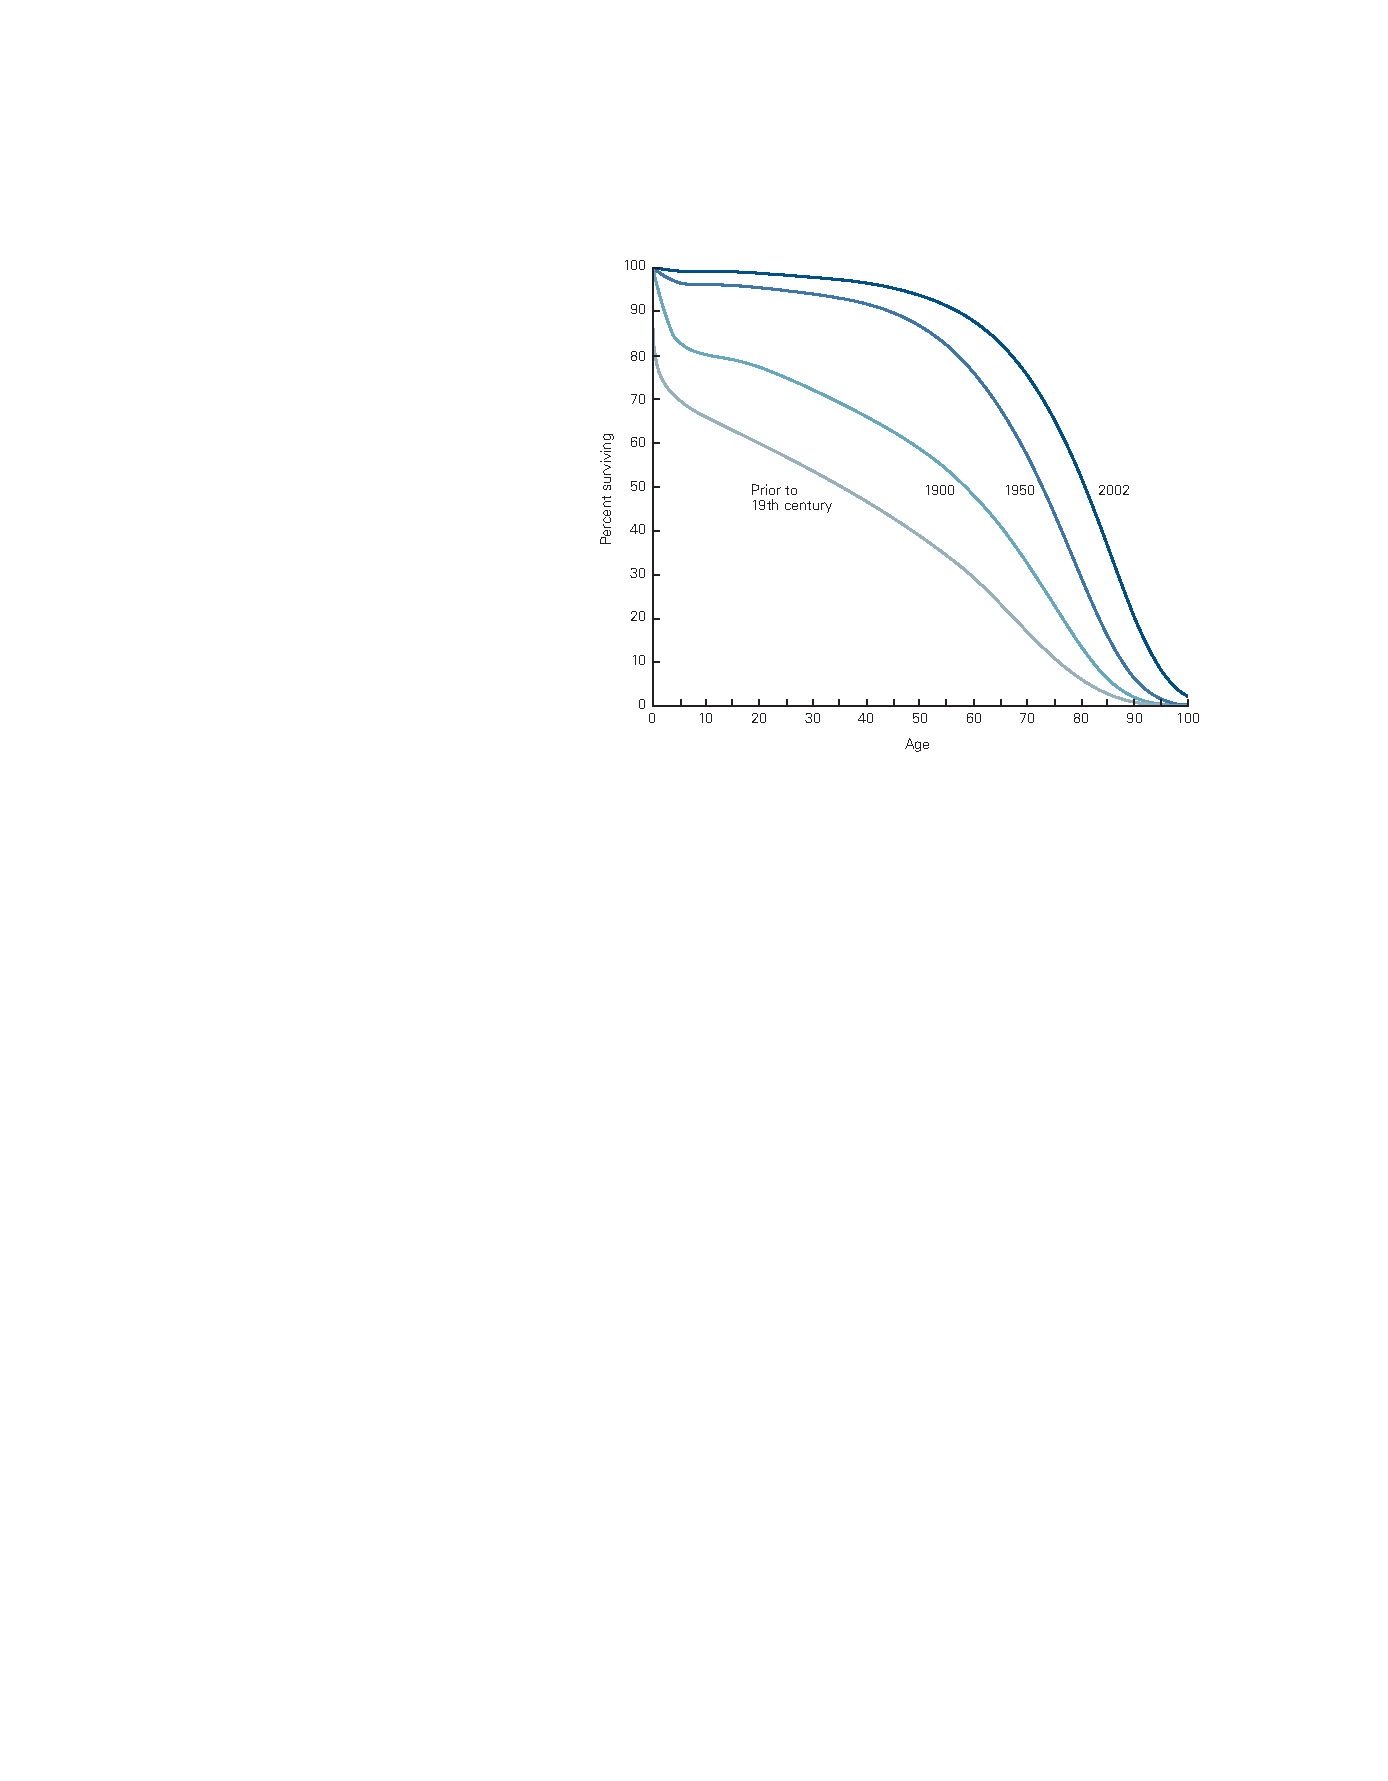
\includegraphics[width=0.7\linewidth]{chap64/fig_64_1}
	\caption{人类的寿命正在增加。 在过去的 100 年里,美国人的平均寿命增长迅速。 (改编自 Strehler 1975;Arias 2004。)}
	\label{fig:64_1}
\end{figure}


寿命延长是一把双刃剑,因为与年龄相关的认知改变越来越普遍。
变化的幅度因人而异。
对于许多人来说,这些改变是温和的,对生活质量的影响相对较小——我们戏称这些短暂的失误称为“老年时刻”。
其他认知障碍虽然不会使人虚弱,但足以阻碍我们独立管理生活的能力。
然而,痴呆症会侵蚀记忆和推理并改变人格。
其中,阿尔茨海默病最为普遍。


随着人口老龄化,神经科学家、神经学家和心理学家开始投入更多精力来了解大脑中与年龄相关的变化。
主要动机是寻找阿尔茨海默病和其他痴呆症的治疗方法,但了解认知能力随年龄下降的正常过程也很重要。
毕竟,年龄是各种神经退行性疾病的最大危险因素。
了解随着年龄的增长我们的大脑会发生什么,不仅可以改善普通人群的生活质量,还可以提供最终帮助我们克服看似无关的病理变化的线索。


考虑到这一点,我们在本章开始考虑大脑的正常老化。
然后我们转向广泛的认知病理变化,最后关注阿尔茨海默病。



\section{大脑的结构和功能随年龄变化}

随着年龄的增长,我们的身体会发生变化——我们的头发变薄,我们的皮肤起皱,我们的关节吱吱作响。
因此,我们的大脑也会发生变化也就不足为奇了。
事实上,随着年龄的增长而发生的广泛行为改变是神经系统潜在改变的迹象。
例如,随着运动技能的下降,姿势变得不那么直立,步态变慢,步幅变短,姿势反射常常变得迟钝。
尽管肌肉变弱并且骨骼变得更脆,但这些运动异常在很大程度上是由涉及周围和中枢神经系统的微妙过程引起的。
睡眠模式也会随着年龄的增长而改变;
老年人睡得更少,醒得更频繁。
归因于前脑的心理功能,例如记忆力和解决问题的能力,也会下降。


与年龄相关的心智能力下降在速度和严重程度上变化很大(图 \ref{fig:64_2}A)。
虽然大多数人的思维敏捷度会逐渐下降,但对某些人来说,下降速度很快,而其他人则终生保持认知能力——朱塞佩·威尔第、埃莉诺·罗斯福和巴勃罗·毕加索就是后一类的著名例子。
提香在 80 年代后期继续创作杰作,据说索福克勒斯在他 92 岁时在科洛诺斯写下了俄狄浦斯。
心理功能完好保存的老年人很少见,这表明这些人的生活经历或基因可能具有特殊性质。
因此,人们对研究在 10 岁甚至 11 岁时几乎保持完好认知的个体产生了极大的兴趣。
这些百岁老人可能会深入了解环境或遗传因素,这些因素可以防止正常的与年龄相关的认知衰退或更具破坏性的痴呆病理下降。
下面讨论的一种保护性基因变体是载脂蛋白 E 基因的 epsilon 2 等位基因。


\begin{figure}[htbp]
	\centering
	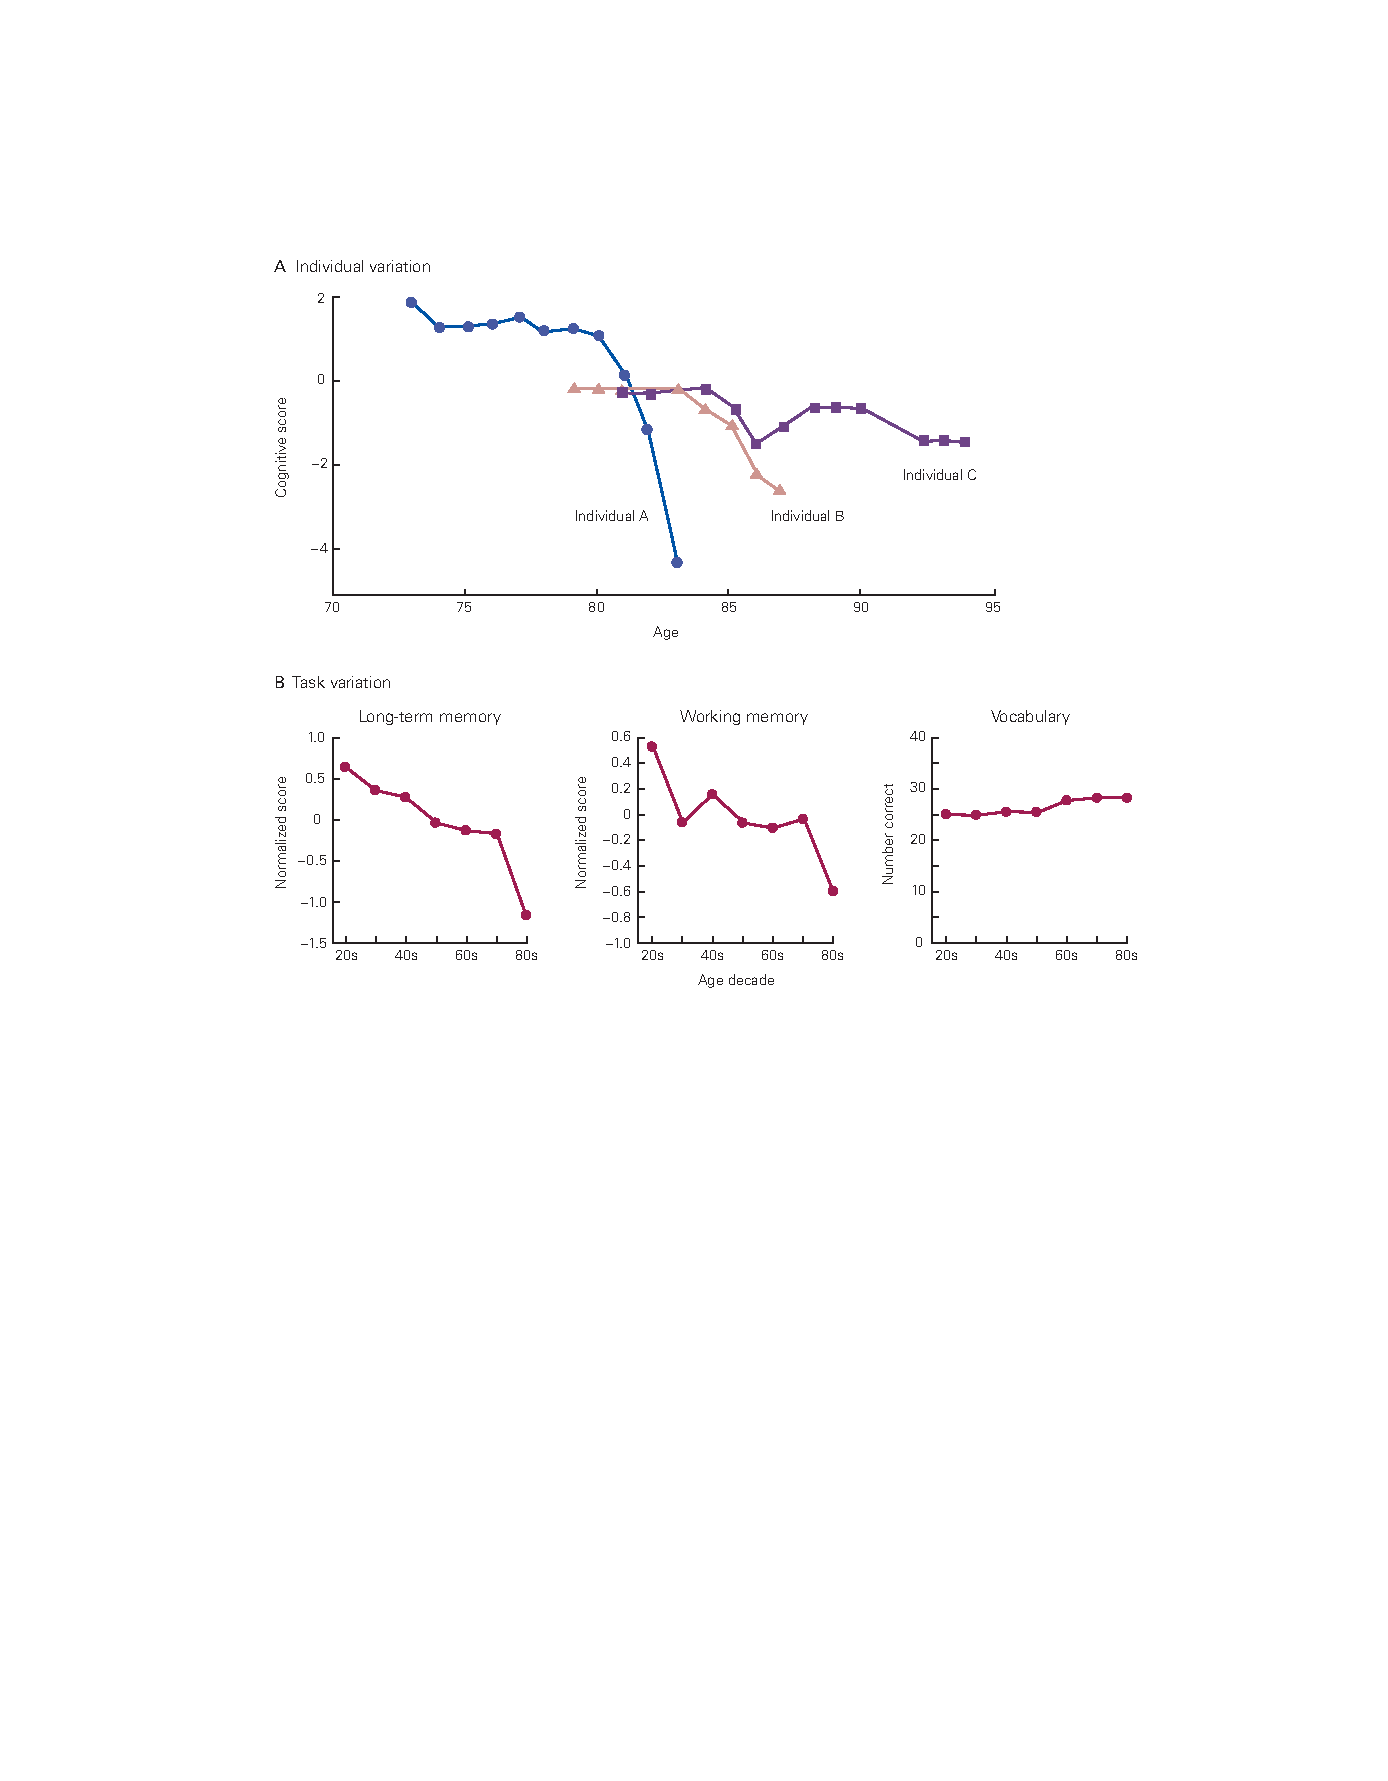
\includegraphics[width=0.8\linewidth]{chap64/fig_64_2}
	\caption{与年龄相关的认知衰退存在差异。 A. 几十年来每年接受一系列认知测试的三个人的分数。 人A迅速下降。 人 B 和 C 在 80 多岁时表现出相似的认知表现,但随后出现分歧。 (改编自 Rubin et al. 1998。) B. 对大量人进行的多项认知测试的平均分数。 长期陈述性记忆和工作记忆在整个生命过程中都会下降,而且在高龄时更是如此。 相反,词汇知识得以保留。 (改编自 Park et al. 1996。)}
	\label{fig:64_2}
\end{figure}


从对许多人的研究中得出的一个有趣发现是,一些认知能力会随着年龄的增长而显着下降,而其他人则基本保持不变(图 \ref{fig:64_2}B)。
例如,工作记忆和长期记忆、视觉空间能力(通过将积木排列到设计中或绘制三维图形来衡量)和语言流畅性(通过快速命名对象或尽可能多地命名以特定字母开头的单词来衡量) ) 通常随着年龄的增长而下降。
另一方面,词汇量、信息和理解力的衡量标准通常显示正常人在进入 80 年代后出现的轻微下降。


记忆力、运动活动、情绪、睡眠模式、食欲和神经内分泌功能的年龄相关变化是由大脑结构和功能的改变引起的。
即使是最健康的 80 岁大脑看起来也不像 20 岁时那样。老年人表现出大脑体积轻度萎缩和脑重量减轻,以及脑室扩大(图 64) –3A)。
从大学时代开始,大脑重量平均每年减少 0.2\%,70 年代每年约减少 0.5\%。


这些变化可能是由神经元死亡引起的。
事实上,一些神经元会随着年龄的增长而丢失。
例如,25\% 或更多支配骨骼肌的运动神经元在一般健康的老年人中死亡。
正如我们将看到的,阿尔茨海默病等神经退行性疾病会显着加速神经元的死亡(图 \ref{fig:64_3}B)。
然而,在健康大脑的大部分区域,仅仅因为年龄的原因,神经元损失很少甚至没有,所以大脑萎缩一定是由其他因素引起的。


\begin{figure}[htbp]
	\centering
	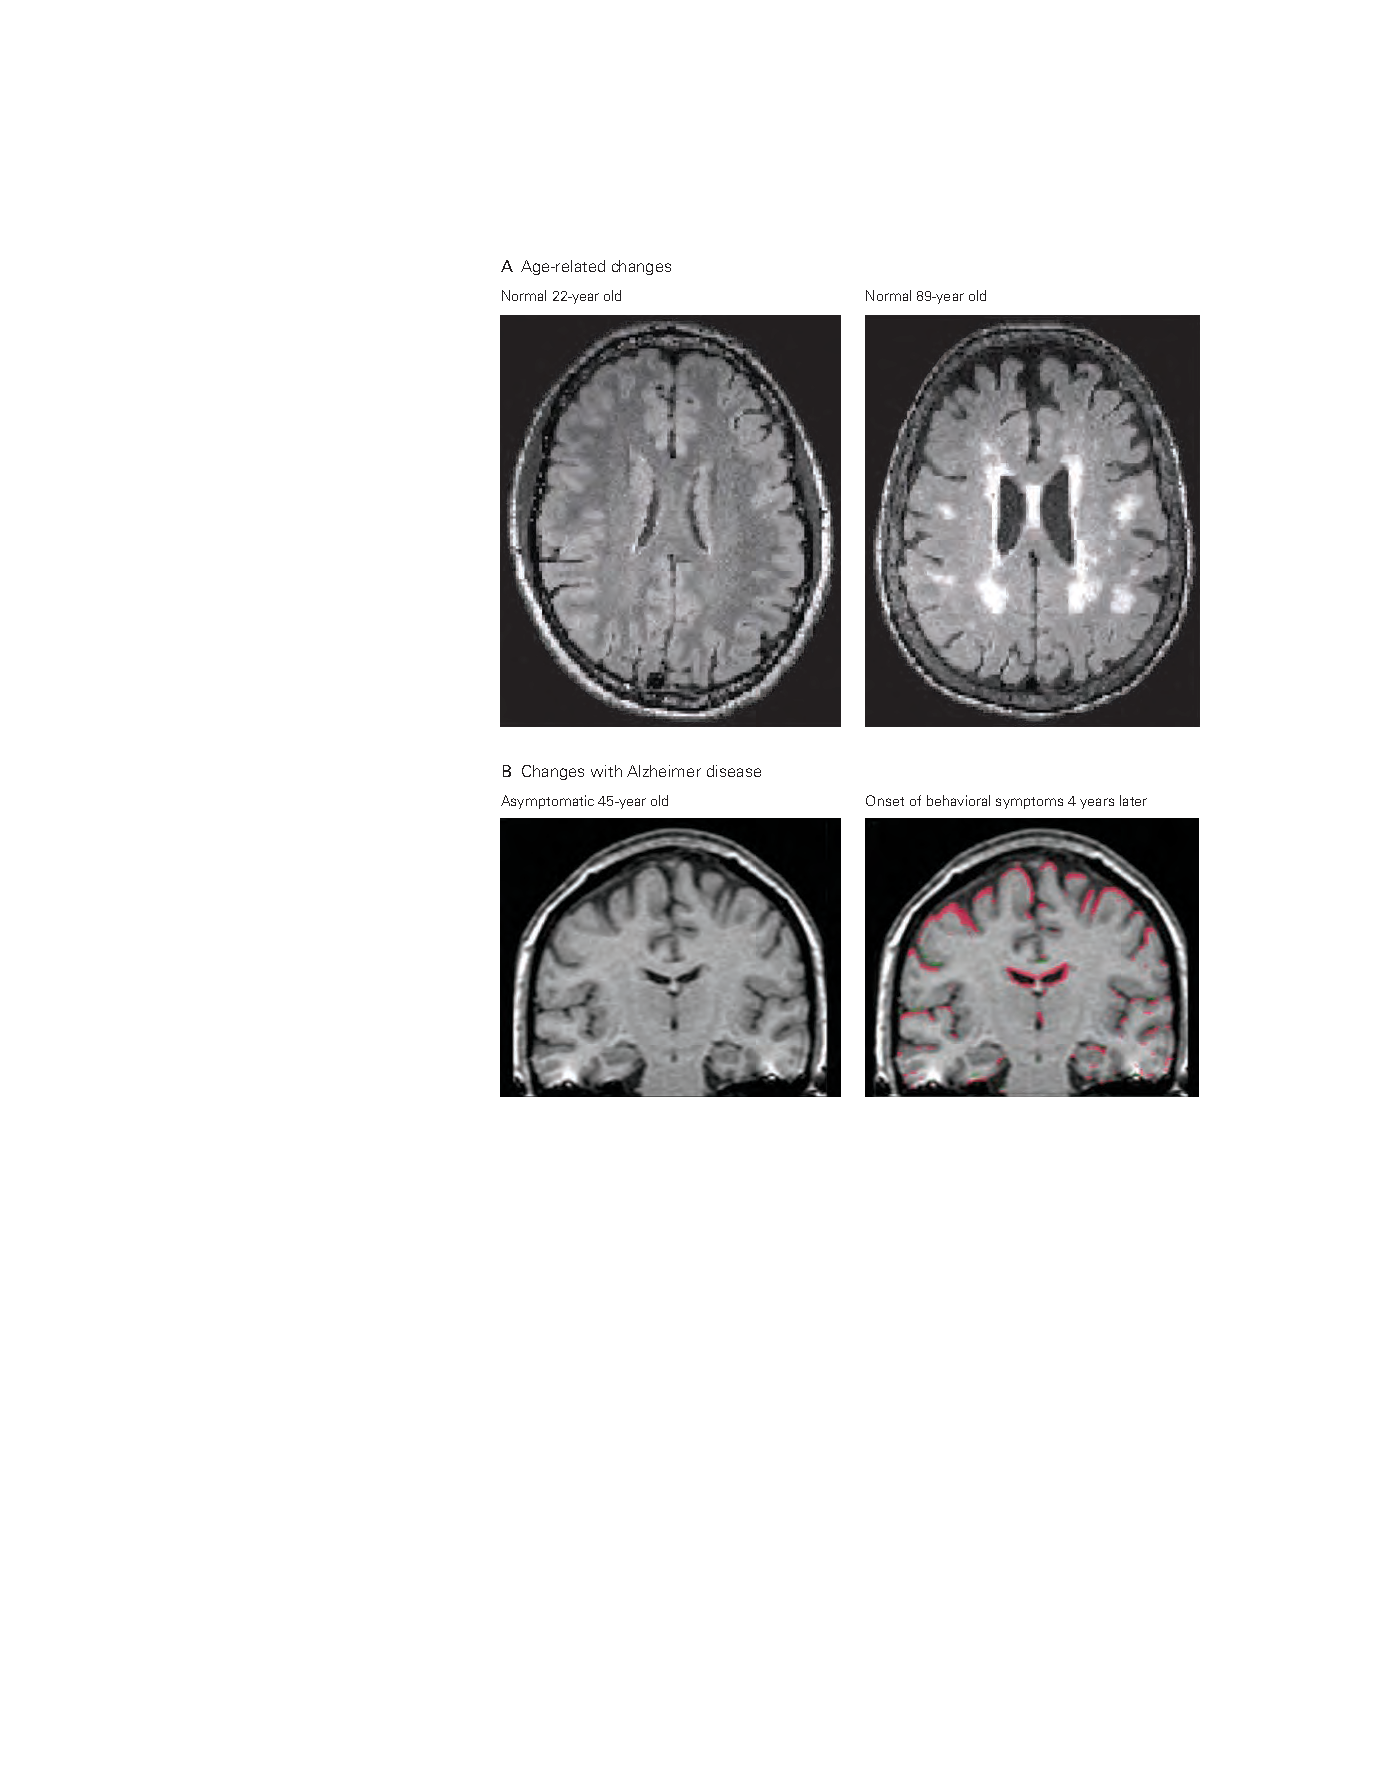
\includegraphics[width=0.7\linewidth]{chap64/fig_64_3}
	\caption{随着年龄的增长和阿尔茨海默病的发作,大脑结构发生变化。 (另请参阅图 \ref{fig:64_8}。) A. 正常 22 岁和 89 岁大脑的图像揭示了活体大脑结构的变化。 (经许可转载自 R. Buckner。) B. 同一个人在 4 年期间的图像显示皮质结构的逐渐收缩和心室扩大的开始(红色)。 这些结构变化在行为症状出现之前就很明显。 (经许可转载自 N. Fox。)}
	\label{fig:64_3}
\end{figure}

事实上,对人类和实验动物大脑的分析揭示了神经元和胶质细胞的结构改变。
髓磷脂破碎和丢失,损害了白质的完整性。
同时,皮质和其他神经元的树突状乔木密度降低,导致神经细胞收缩。
合成某些神经递质(如多巴胺、去甲肾上腺素和乙酰胆碱)的酶水平会随着年龄的增长而下降,这种下降可能会导致使用这些递质的突触出现功能缺陷。
突触结构也发生了改变,至少在神经肌肉接头处是这样(图 \ref{fig:64_4}),增加了结构变化也导致中枢突触功能缺陷的可能性。
最后,新皮质和大脑许多其他区域的突触数量下降(图 \ref{fig:64_5})。


\begin{figure}[htbp]
	\centering
	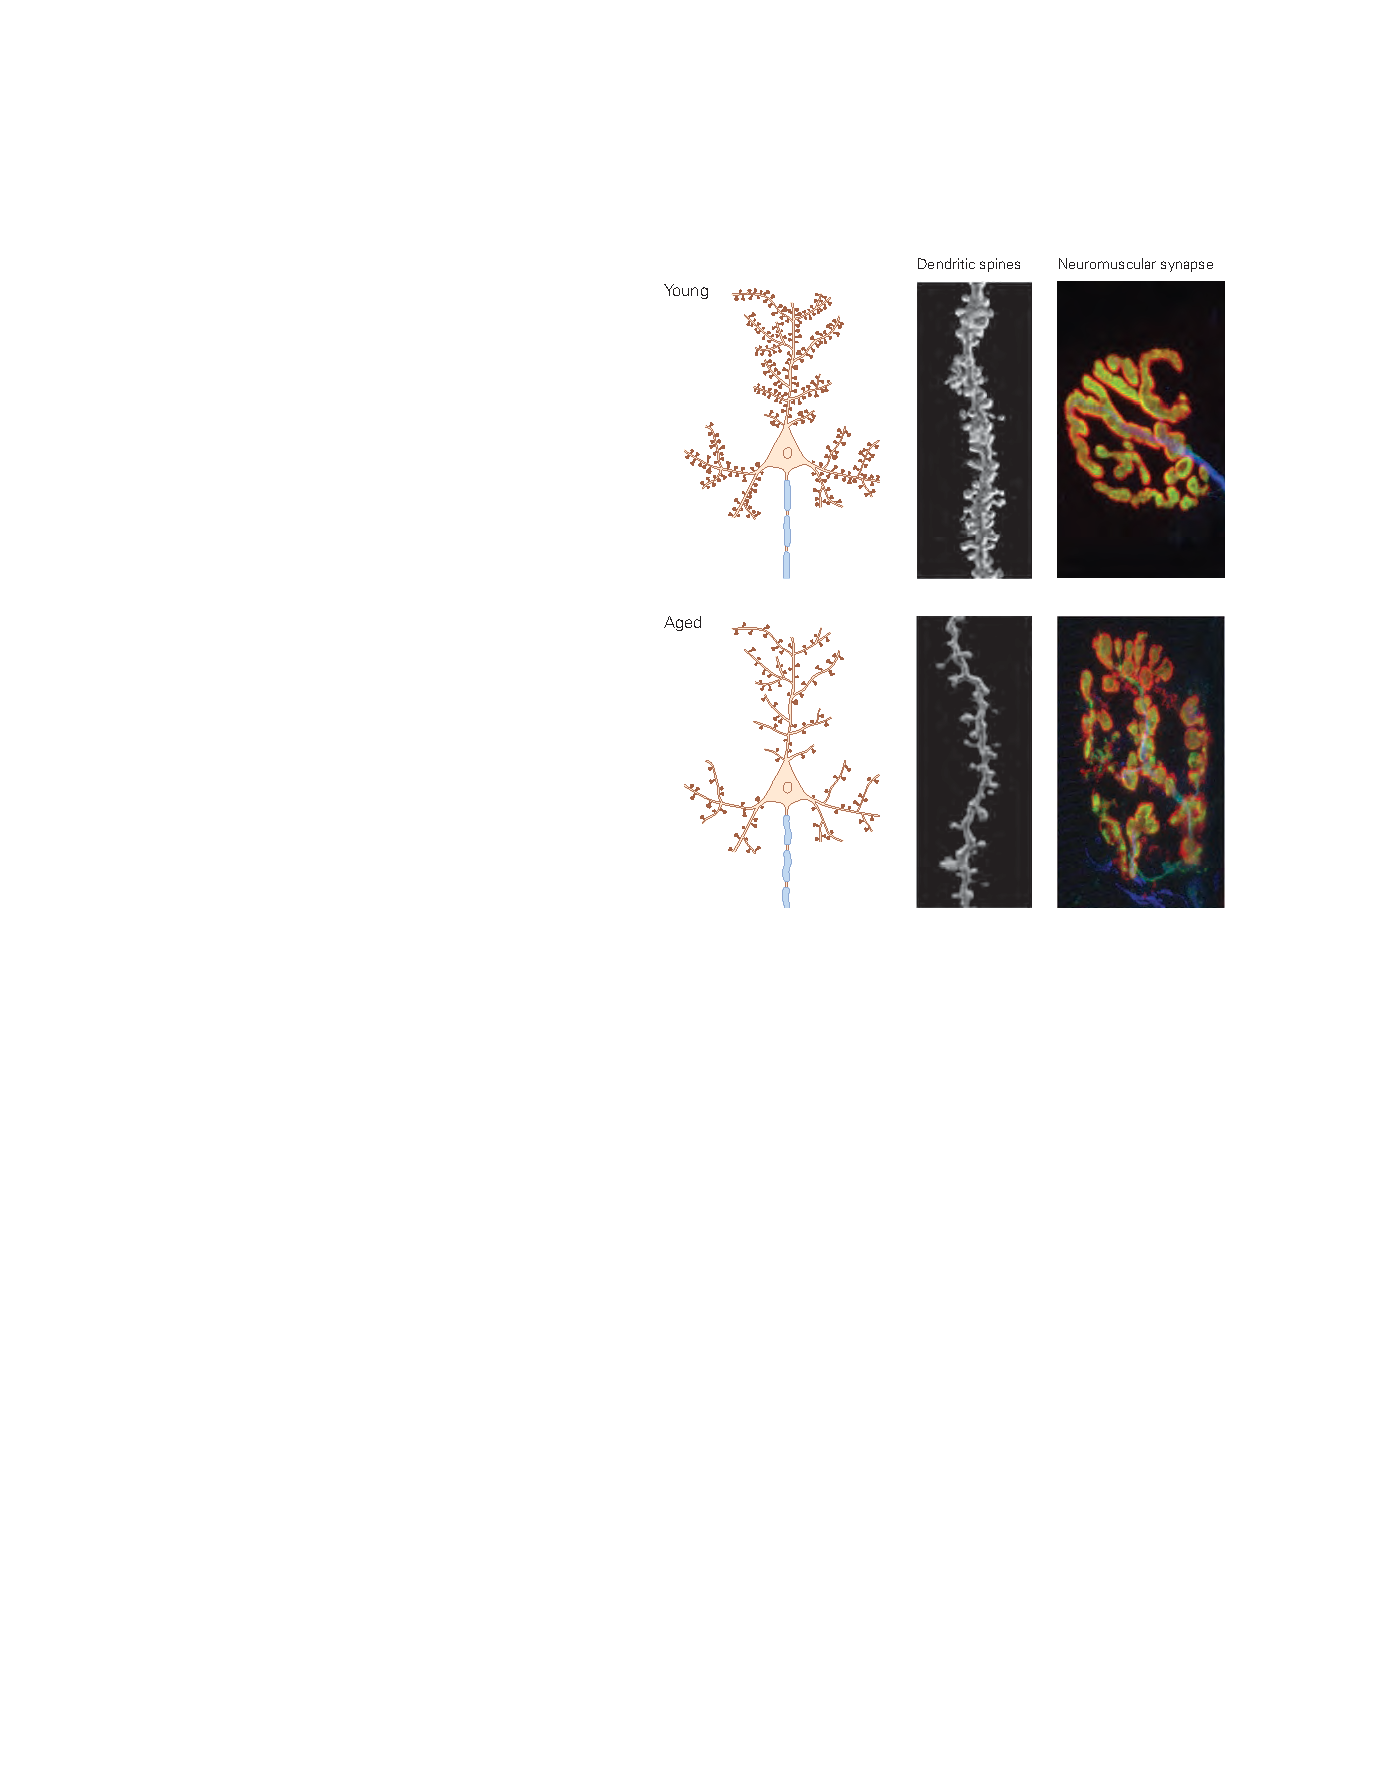
\includegraphics[width=0.6\linewidth]{chap64/fig_64_4}
	\caption{树突和突触结构与年龄相关的变化。 啮齿动物的皮质锥体神经元随着年龄的增长而失去树突棘。 啮齿动物的神经肌肉突触也表现出与年龄相关的结构变化。 (经许可转载自 J. Luebke 的脊柱图像;经许可转载自 G. Valdez 的突触图像。)}
	\label{fig:64_4}
\end{figure}

\begin{figure}[htbp]
	\centering
	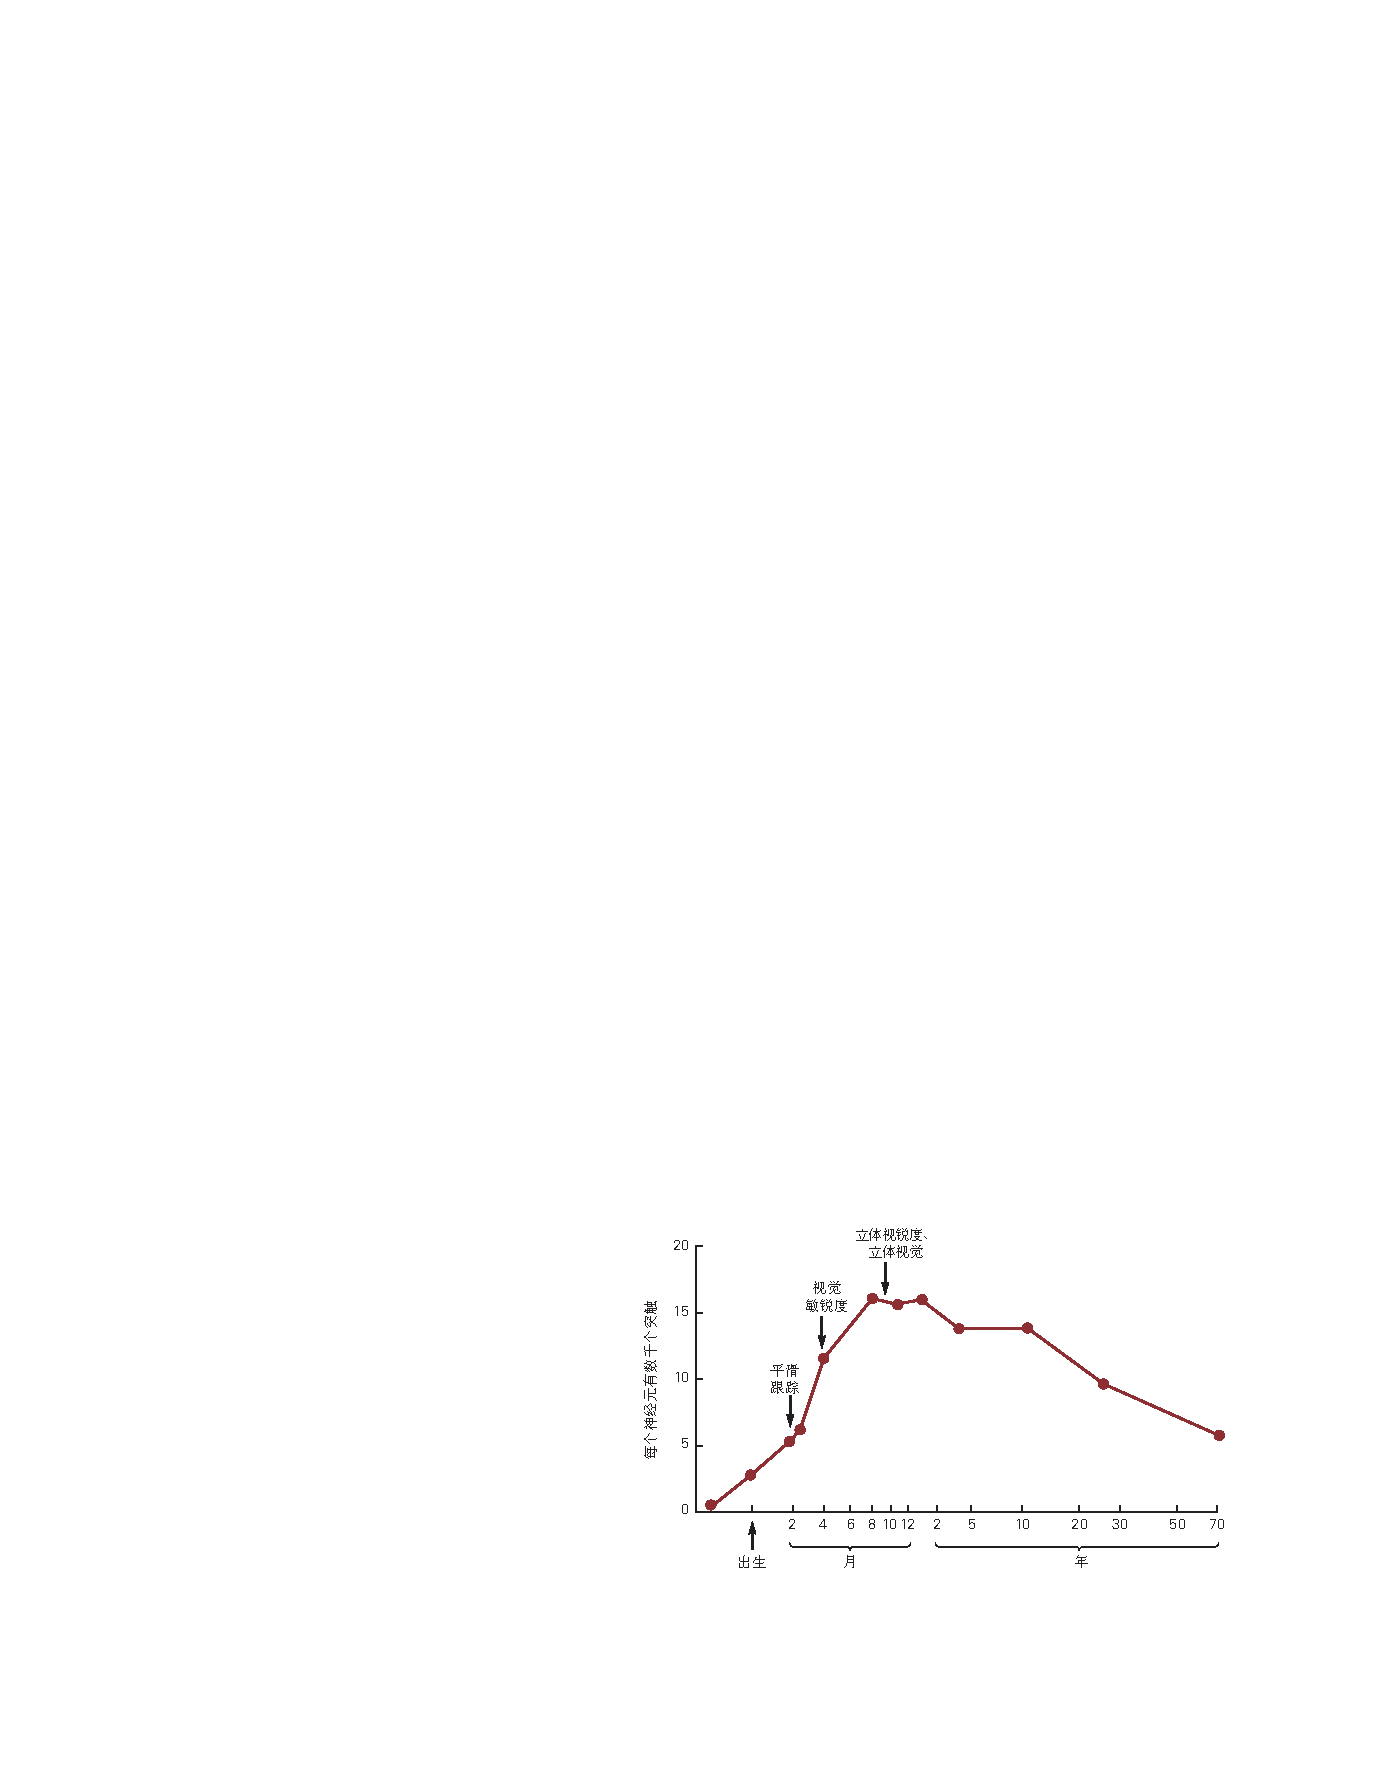
\includegraphics[width=0.6\linewidth]{chap64/fig_64_5}
	\caption{突触密度与年龄相关的变化。 早期认知发展伴随着人类大脑皮层不同区域突触密度的显着增加。 显示了 10 个月大的发育标志。 皮质突触的密度随着年龄的增长而下降。 (改编自 Huttenlocher 2002。)}
	\label{fig:64_5}
\end{figure}

这些细胞变化会干扰调节我们心理活动的神经回路的完整性。
与年龄相关的突触丧失以及剩余突触功能受损被认为是导致认知能力下降的重要因素。
白质的变化很普遍,但在前额叶和颞叶皮层尤为显着。
它们可能是执行功能和集中注意力以及编码和存储记忆的能力改变的基础,这些功能位于额叶-纹状体系统和颞叶中。
白质的损失也可能有助于解释最近的发现,即老年人的大脑不太能够支持通常协同工作以进行复杂心理活动的广泛分离区域的活动同步。
这些大规模网络的中断可能是认知能力下降的重要原因。


长期以来,人们一直认为衰老是由于累积的遗传损伤或有毒废物导致细胞和组织逐渐退化的结果。
支持这一想法的发现是,从动物身上取出并置于组织培养皿中的有丝分裂细胞在衰老和死亡之前仅分裂有限次数。
这种“注定”衰老的观点在过去 10 到 20 年里发生了根本性的变化,这主要是由于在模式生物中发现了显着延长寿命的突变(图 \ref{fig:64_6})。


\begin{figure}[htbp]
	\centering
	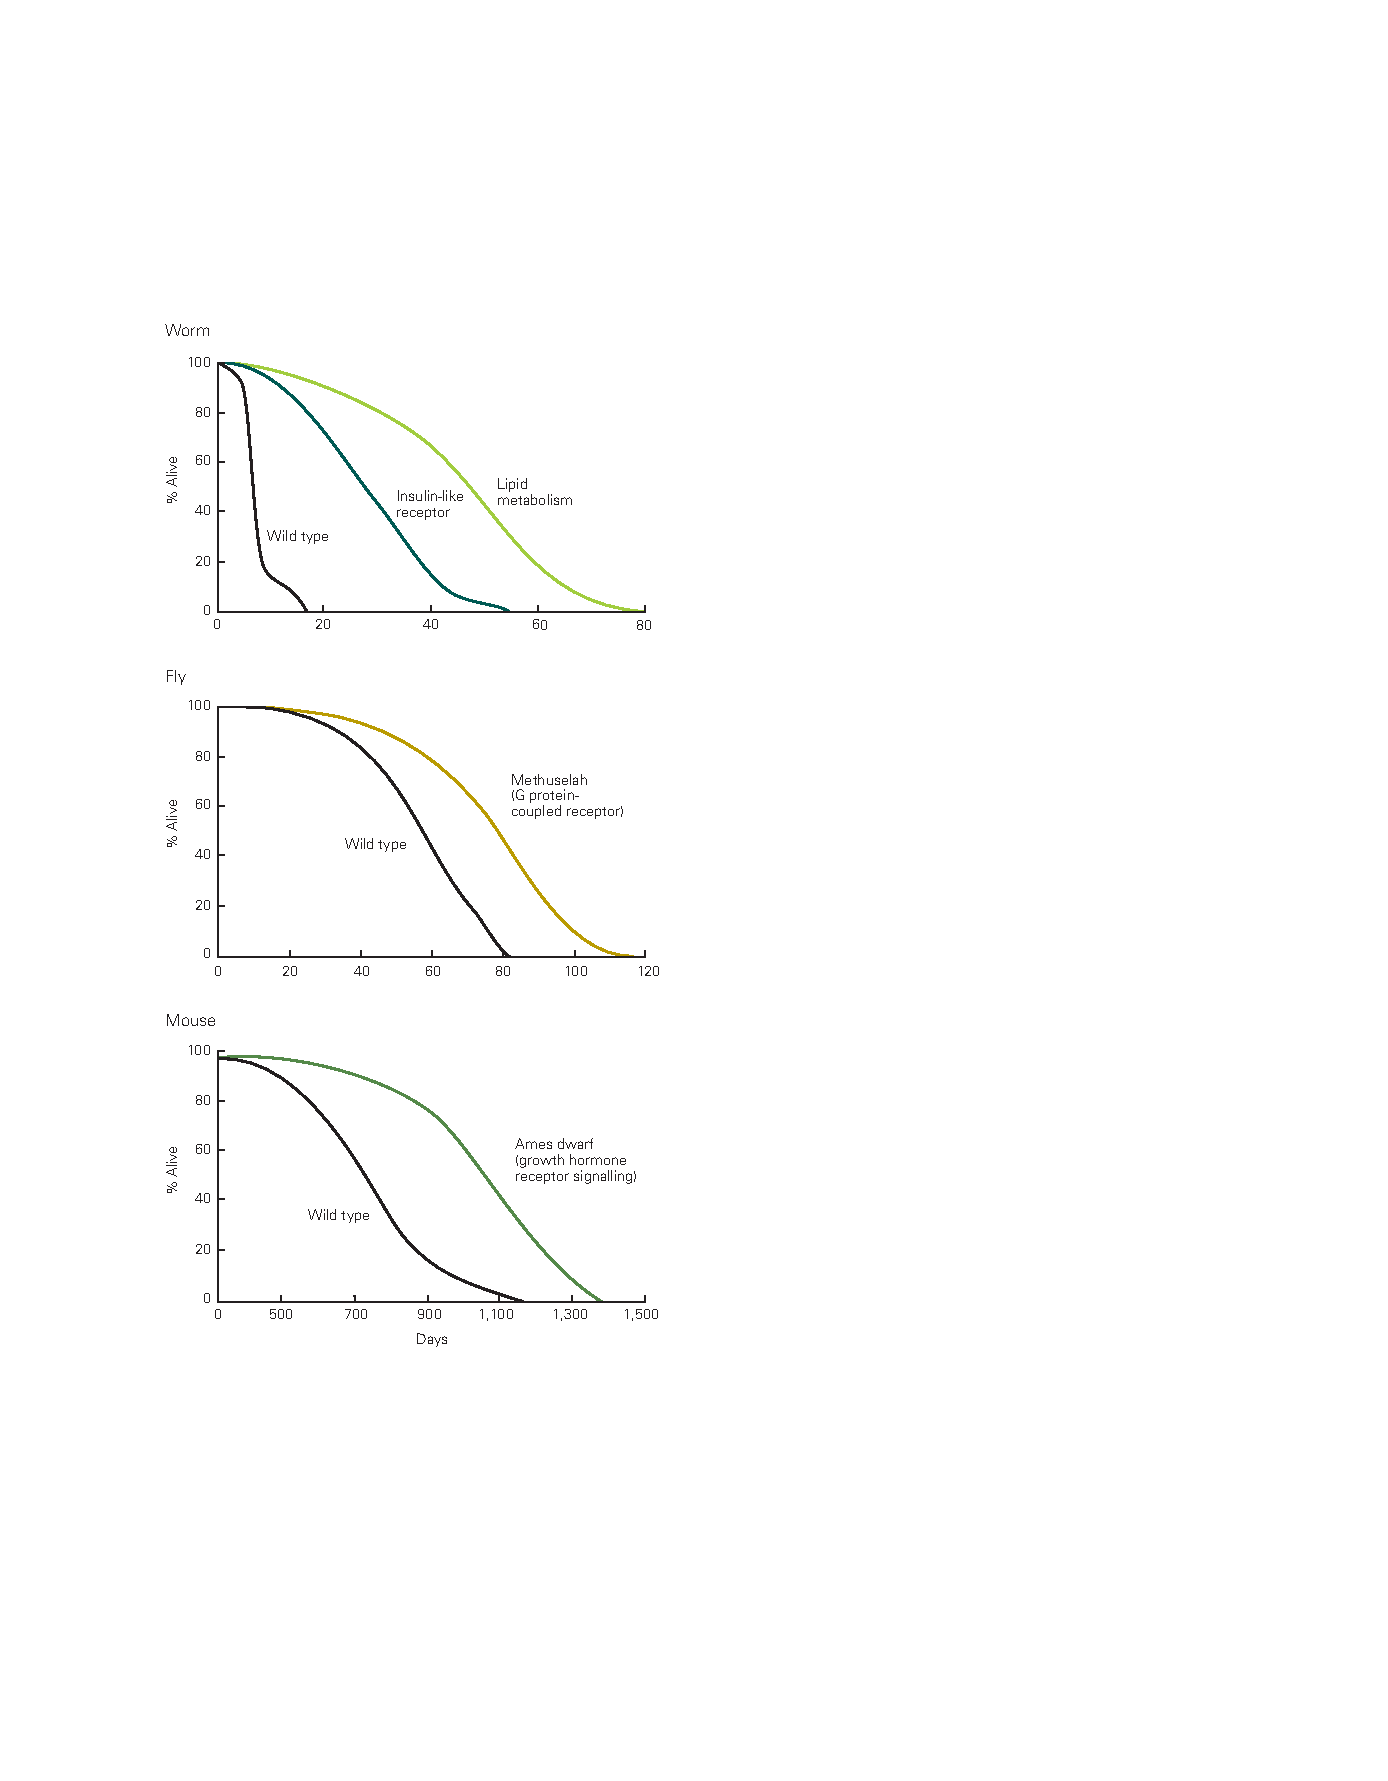
\includegraphics[width=0.5\linewidth]{chap64/fig_64_6}
	\caption{寿命可以通过基因突变来增加。 特定受体和信号蛋白的基因突变显着延长了蠕虫、苍蝇和小鼠突变株的寿命,表明遗传调节机制影响衰老和寿命。 (上图改编自 Hekimi 和 Guarente 2003;中间经许可转载自 Yi、Seroude 和 Benzer 1998。版权所有 © 1998 AAAS;下图改编自 Brown-Borg 等人,1996。)}
	\label{fig:64_6}
\end{figure}


这些戏剧性的发现表明,衰老过程是在积极的基因控制下进行的。
一种已被表征的调节途径包括胰岛素和胰岛素样生长因子、它们的受体以及它们激活的信号传导程序。
这些基因的破坏实际上增加了细胞对致命氧化损伤的抵抗力。
人们认为,这些基因的正常形式是通过进化选择的,因为它们在生殖期对生物体有益。
一旦动物过了生育年龄,它们对长寿的有害影响可能是一种不幸的副作用,而进化并不关心。


这些发现对于理解衰老如何影响神经系统有两个主要意义。
首先,导致或保护我们免受年龄破坏的生化机制很可能是导致与年龄相关的认知能力下降的神经元变化的原因。
探索细胞变化与认知功能之间这种联系的研究目前正在模式生物中进行。
其次,也许更令人兴奋的是,对基因研究发现的途径的研究可以确定延长寿命或健康寿命(一个人保持总体健康的时期)的药理学或环境策略。


迄今为止,延长寿命(从酵母到蠕虫再到灵长类动物)的最佳验证环境策略是热量限制。
热量限制似乎是通过上述胰岛素通路中的基因起作用的,并且可能涉及一组称为 sirtuins 的酶。
sirtuins 被最初从红酒中分离出来的化合物白藜芦醇激活。
当给小鼠服用时,白藜芦醇反过来会延缓衰老的某些方面,包括认知能力下降。
虽然白藜芦醇不太可能成为人类的青春之泉,但它仍然是目前正在考虑的新化学物质的例证。
这些化学策略不仅使用模式生物探索导致衰老的积极因素,而且探索阻止模式生物(可能还有人类)在其整个生命周期中保持总体健康的限制因素。



\section{相当一部分老年人的认知能力下降是显着的并且使人虚弱}

对于大多数人来说,与年龄相关的认知变化不会严重影响生活质量。
然而,在一些老年人中,认知能力下降达到了可以被视为病态的程度。
在异常范围的低端是一系列称为轻度认知障碍 (MCI) 的变化。
这种综合征的特征是记忆力减退,伴有或不伴有其他认知障碍,这些障碍超出了正常衰老的范围。
患有 MCI 的人可能能够进行大多数日常生活活动,尽管其他人会注意到这些损伤,并且通常会影响受影响的人进行某些对他们来说重要或愉快的活动的能力,例如管理财务或玩游戏 文字游戏。


重要的是,MCI 是一种综合征,而不是一种诊断。
许多潜在的问题,如抑郁症、过度用药、中风和神经退行性疾病都可能导致 MCI。
大约一半的 MCI 患者患有潜在的阿尔茨海默病,并且该组中超过 90\% 的人将在 MCI 诊断后的 5 年内发展为完全痴呆(图 \ref{fig:64_7})。
如下所述,现在有生物标志物可以提示潜在的阿尔茨海默病病理学的存在。
然而,到目前为止,还没有很好的生物标志物来预测由阿尔茨海默病以外的疾病引起的 MCI 患者进展为痴呆症。


\begin{figure}[htbp]
	\centering
	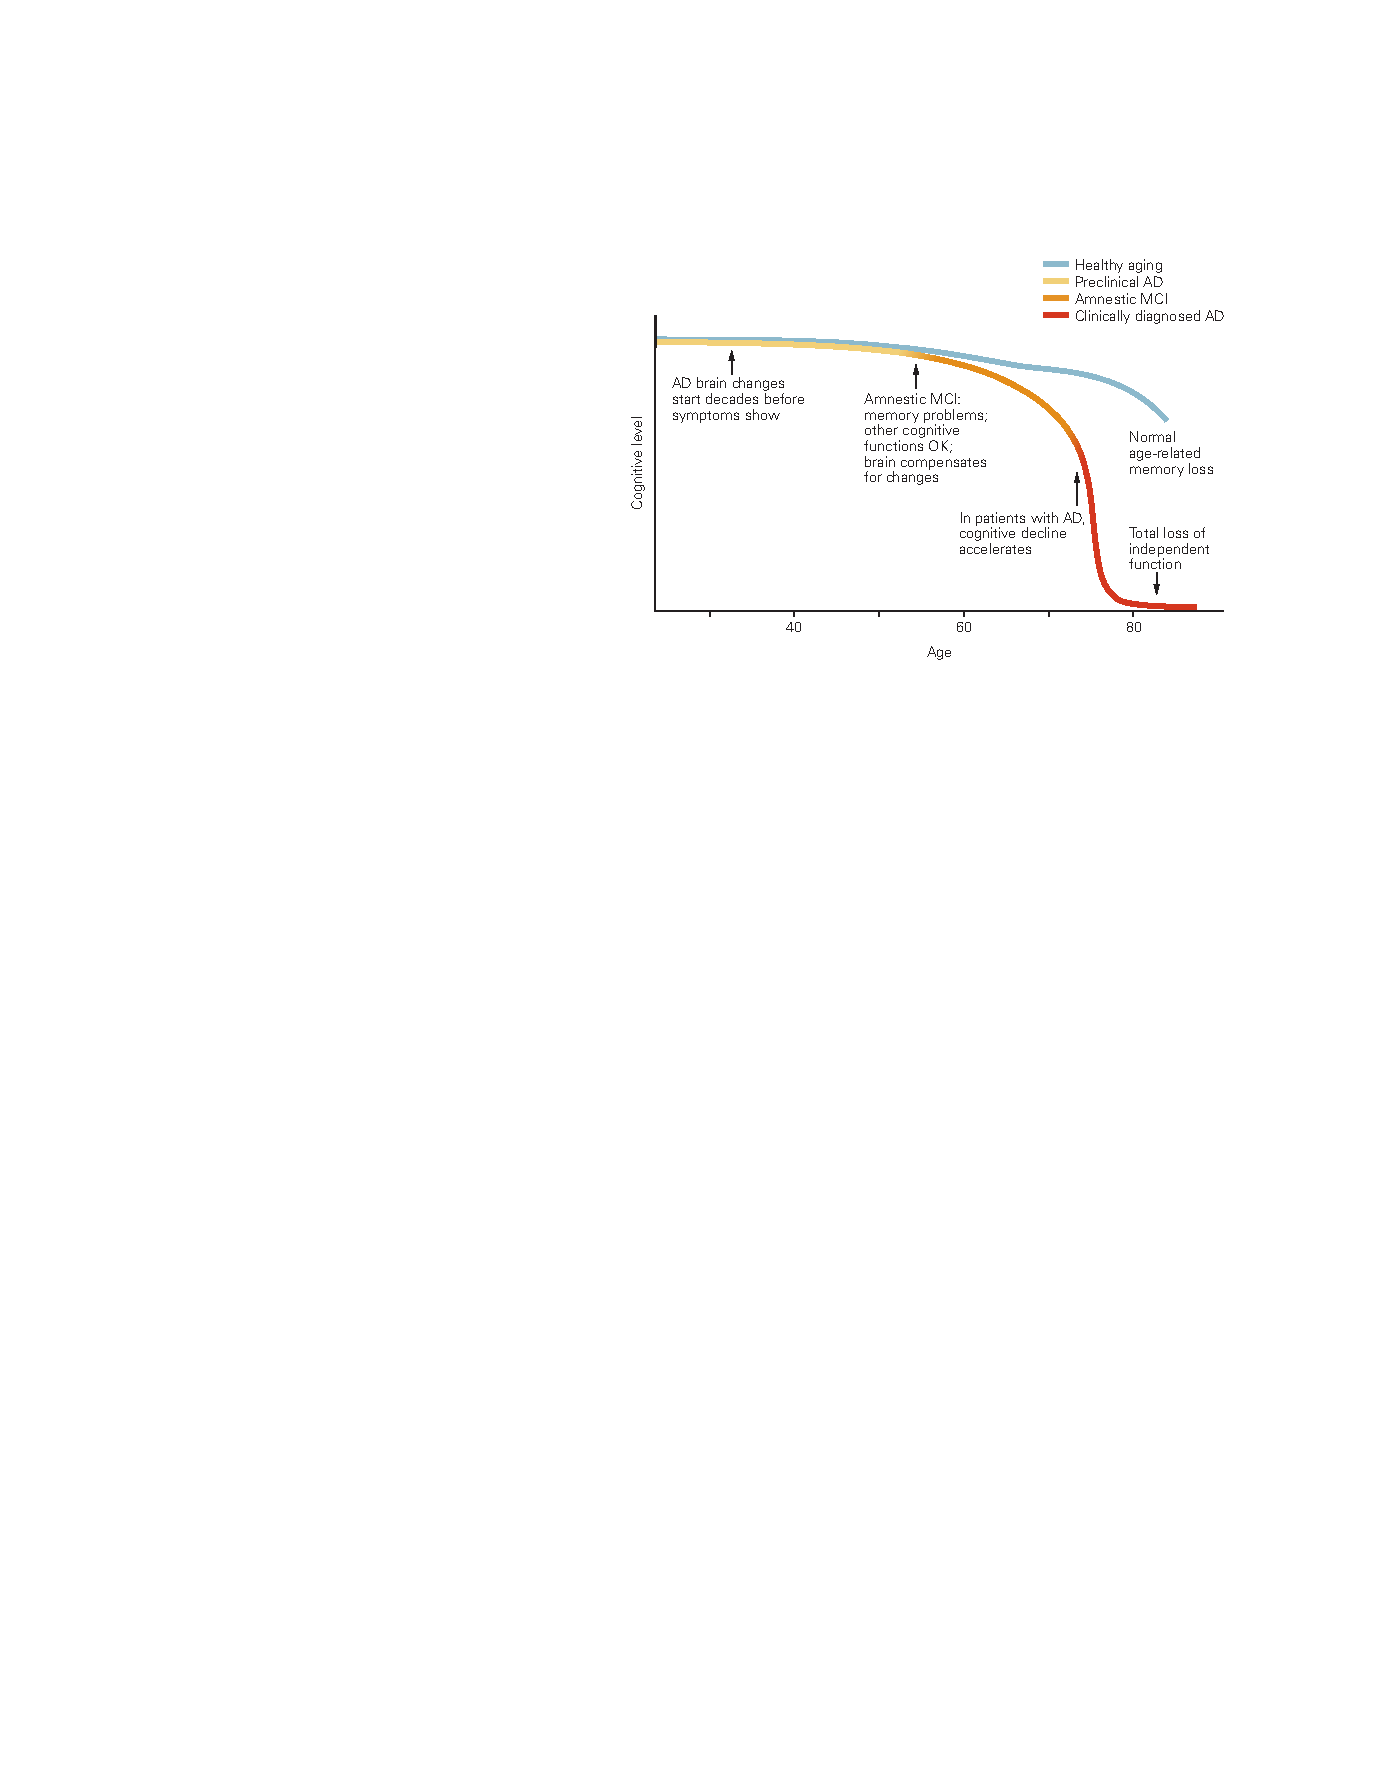
\includegraphics[width=0.6\linewidth]{chap64/fig_64_7}
	\caption{认知能力随年龄变化很大。 该图表显示了当前对阿尔茨海默病 (AD) 病因的思考。 这个渐进的过程是由生物、遗传、环境和生活方式因素共同作用的结果,最终使一些人走上轻度认知障碍 (MCI) 的道路,然后是痴呆症。 其他人,在一生中具有不同的基因构成或不同的因素组合,继续健康的认知老化过程。 (来自国家老龄化研究所:http://www.nia.nih.gov/alzheimers/publication/part-2-what-happens-brain-ad/changing-brain-ad。)}
	\label{fig:64_7}
\end{figure}


与 MCI 一样,痴呆症也是一种涉及记忆力以及其他认知能力(如语言、问题解决、判断、计算或注意力)进行性损害的综合症。
它与多种疾病有关。 最常见的是阿尔茨海默病,如下所述。
老年人中第二个最常见的原因是脑血管疾病,特别是导致局灶性缺血和随之而来的脑梗塞的中风。


皮质中的大损伤通常与语言障碍(失语症)、偏瘫或忽视综合征有关,具体取决于大脑的哪些部分受到损害。
白质或大脑深层结构中的小梗死,称为腔隙性腔隙,也是高血压和糖尿病的结果。
在少数情况下,这些梗塞可能没有症状,或者它们可能导致看似正常的与年龄相关的认知能力下降或某些 MCI 病例。
然而,随着血管病变数量和大小的增加,它们的影响会累积,最终会导致痴呆。


许多其他情况可导致痴呆,包括帕金森病、路易体痴呆、额颞叶痴呆、酒精中毒、药物中毒、艾滋病毒和梅毒等感染、脑肿瘤、硬膜下血肿、反复脑外伤、维生素缺乏症(尤其是缺乏维生素 B12) 、甲状腺疾病和各种其他代谢紊乱。
反复的脑外伤会导致所谓的慢性创伤性脑病 (CTE)。
最近报道了许多美国职业运动员的 CTE 病例。 在一些患者中,精神分裂症或抑郁症可能类似于痴呆症。
(Emil Kraepelin 选择术语“早发性痴呆”来描述我们现在称为精神分裂症的认知疾病。)由于某些痴呆症是可以治疗的,因此医生根据临床病史、体格检查和身体状况来探查痴呆症的鉴别诊断非常重要。 实验室研究。



\section{阿尔茨海默病是痴呆症最常见的原因}

1901 年,Alois Alzheimer 检查了一名逐渐丧失认知能力的中年妇女。
她的记忆力越来越差。
她再也无法辨别方向,即使是在自己家里,她也把东西藏在了自己的公寓里。
有时,她认为人们打算谋杀她。


她被送进了一家精神病院,并在阿尔茨海默博士第一次见到她大约 5 年后去世。
死后,阿尔茨海默进行了尸检,揭示了大脑皮层的特定改变,如下所述。
一系列行为症状和身体改变随后被命名为阿尔茨海默病 (AD)。


这个病例引起了老年痴呆症的注意,因为它发生在中年; AD 的最初临床表现(通常是记忆力减退和执行功能下降)最常出现在 65 岁以后。
70 岁时 AD 的患病率约为 2\%,而 80 岁后则超过 20\%。
65 岁之前的早发病例通常是家族性的(常染色体显性遗传性 AD),并且已经在其中许多患者中发现了基因突变,我们将在下面讨论。
事实上,最近对第一例阿尔茨海默病患者保存的大脑样本进行的新基因测试表明,她的疾病是由一种叫做早老素-1 的基因突变引起的,这是家族性或显性遗传性 AD 的最常见原因。
迟发性 AD(65 岁或以上发病)通常是散发性的,这意味着不存在显性遗传性 AD 中出现的单一致病基因。
尽管如此,很明显,遗传学甚至更可能通过影响易感性的变异,以及刚刚被发现的环境和其他促成因素,对晚发性 AD 的风险做出巨大贡献。


AD 的早发型和晚发型类型通常都表现出情景记忆和执行功能的选择性缺陷。
起初,语言、力量、反应、感觉能力和运动技能几乎正常。
然而,记忆和注意力会逐渐丧失,连同解决问题、语言、计算和视觉空间感知等认知能力也会丧失。
不出所料,这些认知丧失会导致行为改变,一些患者会出现幻觉和妄想等精神病症状。
所有患者均出现精神功能和日常生活活动进行性损害;
在晚期阶段,他们变得哑巴、大小便失禁和卧床不起。


阿尔茨海默病影响大约八分之一的 65 岁以上老年人。 现在美国有超过 500 万人因 AD 而患上痴呆症。
由于老年人口快速增加,AD风险人群也在快速增长。
在接下来的 25 年里,美国患有 AD 的人数预计将增加两倍,照顾不再能够照顾自己的患者的费用也将增加三倍。
因此,AD是社会的主要公共卫生问题之一。



\section{阿尔茨海默病患者的大脑因萎缩、淀粉样斑块和神经原纤维缠结而改变}

在 AD 中发现了三类大脑异常。
首先,由于神经元和突触丢失,大脑萎缩,脑回变窄,脑沟变宽,脑重量减轻,脑室扩大(图 \ref{fig:64_8})。
这些变化也以较轻微的形式出现在因其他原因死亡的认知完好老年人身上。
因此,AD是一种神经退行性疾病。


\begin{figure}[htbp]
	\centering
	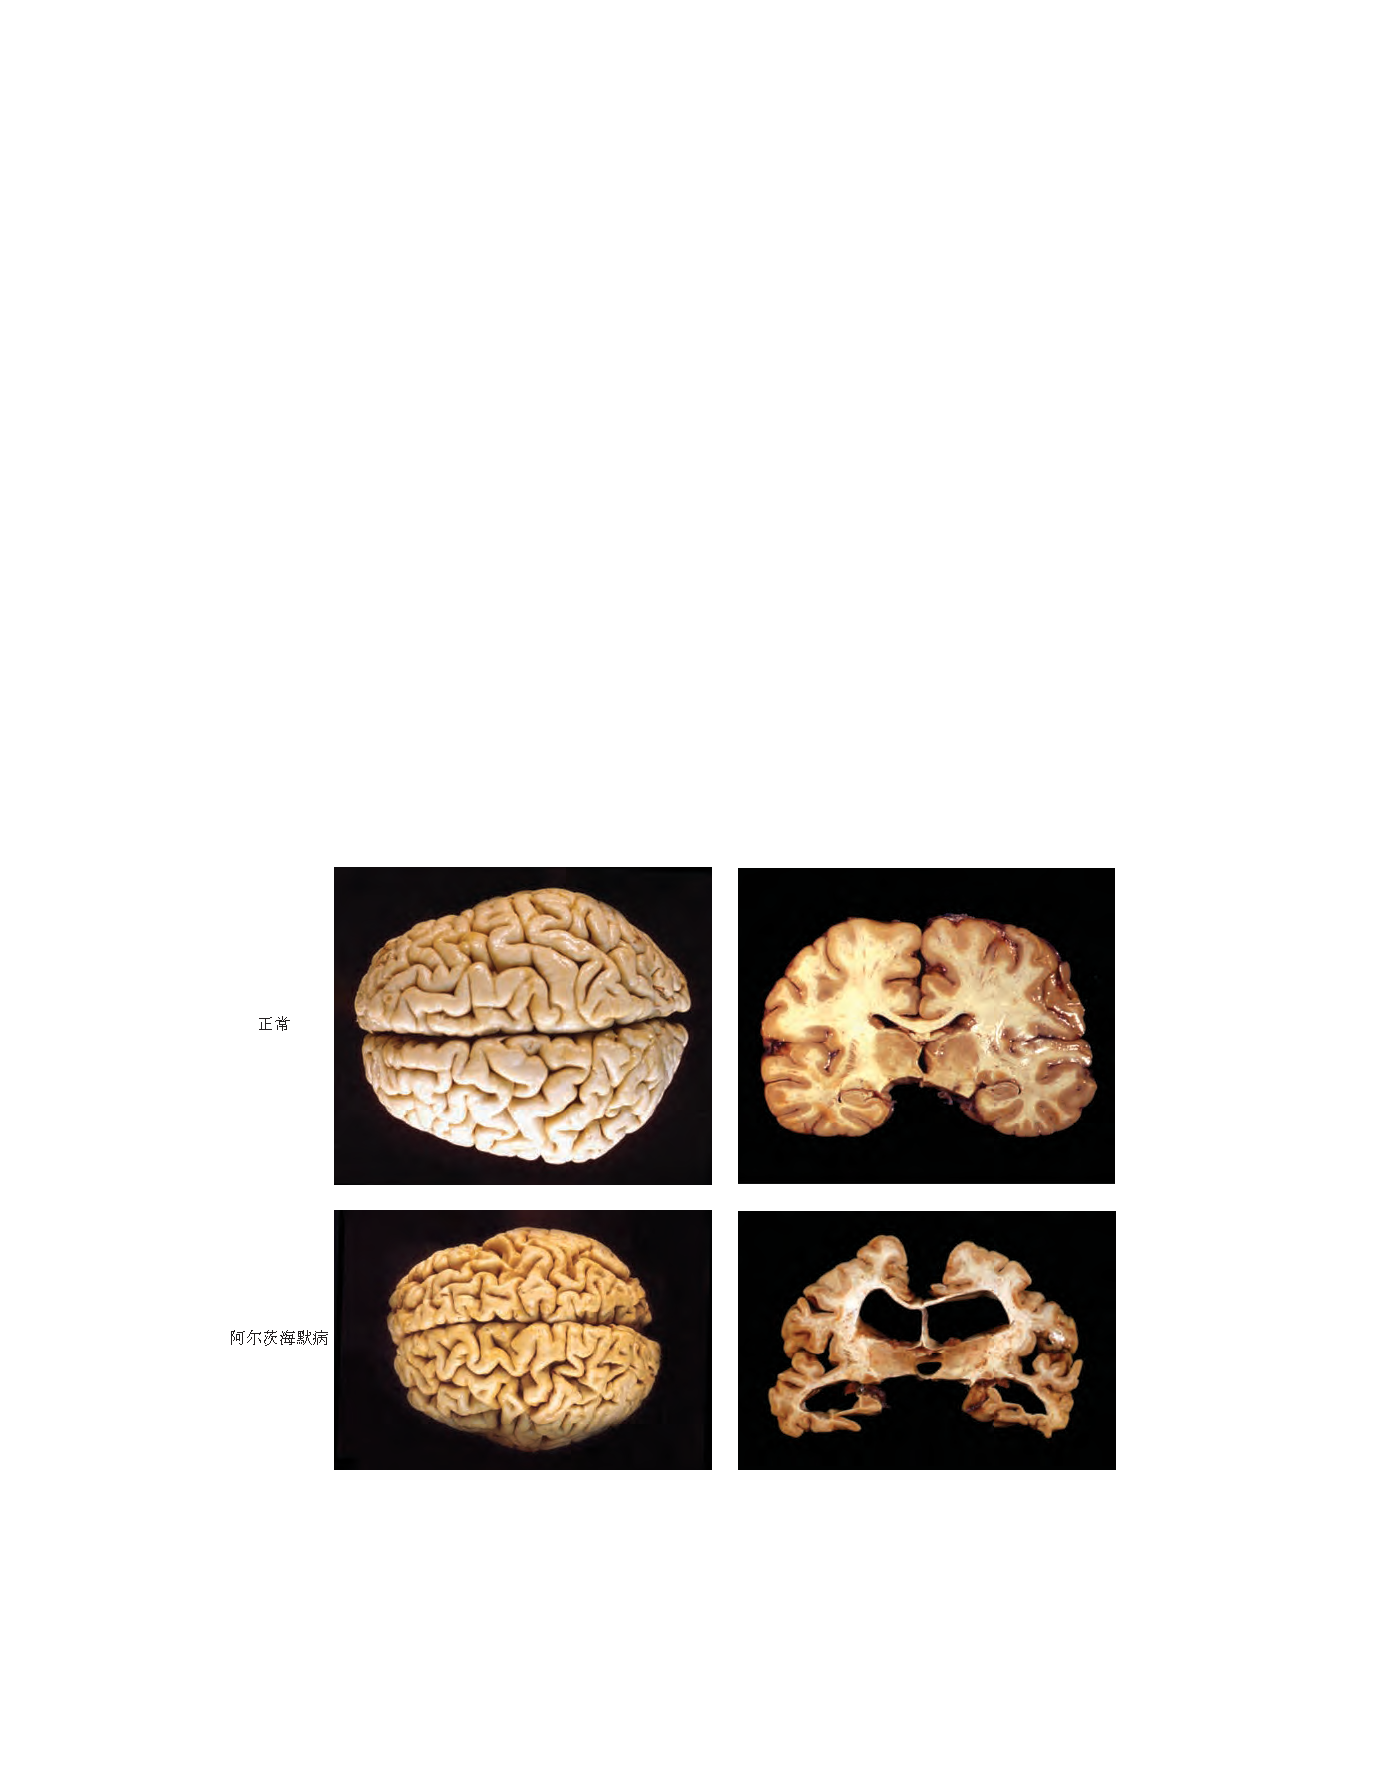
\includegraphics[width=0.8\linewidth]{chap64/fig_64_8}
	\caption{阿尔茨海默病患者大脑的明显病理变化。 与年龄匹配的正常大脑相比,阿尔茨海默病患者的大脑显示出明显的萎缩和脑室扩大。 (另请参见图 64-3。)(经许可转载自阿拉巴马大学伯明翰分校病理学系的全脑照片 © PEIR 数字图书馆 [http://peir.net];经许可转载的脑切片照片来自 A.C. 麦基。)}
	\label{fig:64_8}
\end{figure}


其次,AD 患者的大脑含有主要由聚集形式的称为淀粉样蛋白-β 或 Aβ 的肽组成的细胞外斑块,它是从正常产生的蛋白质中切割下来的。
Aβ 的聚集体称为淀粉样斑块。 斑块中的大部分 Aβ 是纤维状的;
Aβ 的聚集体与其他与 Aβ 共聚集的蛋白质一起出现在 β 折叠片构象中(图 \ref{fig:64_9})。
当用刚果红等染料染色时,淀粉样蛋白可以被检测到,当在偏振光下观察时,或者当用硫黄素 S 染色并用荧光光学器件观察时,淀粉样蛋白是折射的。
淀粉样蛋白的细胞外沉积物被肿胀的轴突和树突包围(神经炎性营养不良)。
这些神经元过程又被激活的星形胶质细胞和小胶质细胞(炎症细胞)的细胞过程所包围。
Aβ 还可以在大脑小动脉壁形成淀粉样沉积物,产生所谓的脑淀粉样血管病。
这在高达 90\% 的 AD 患者中不同程度地发生,但它也可以独立于 AD 发生。
脑淀粉样血管病可导致缺血性中风,是老年人出血性中风的常见原因。


\begin{figure}[htbp]
	\centering
	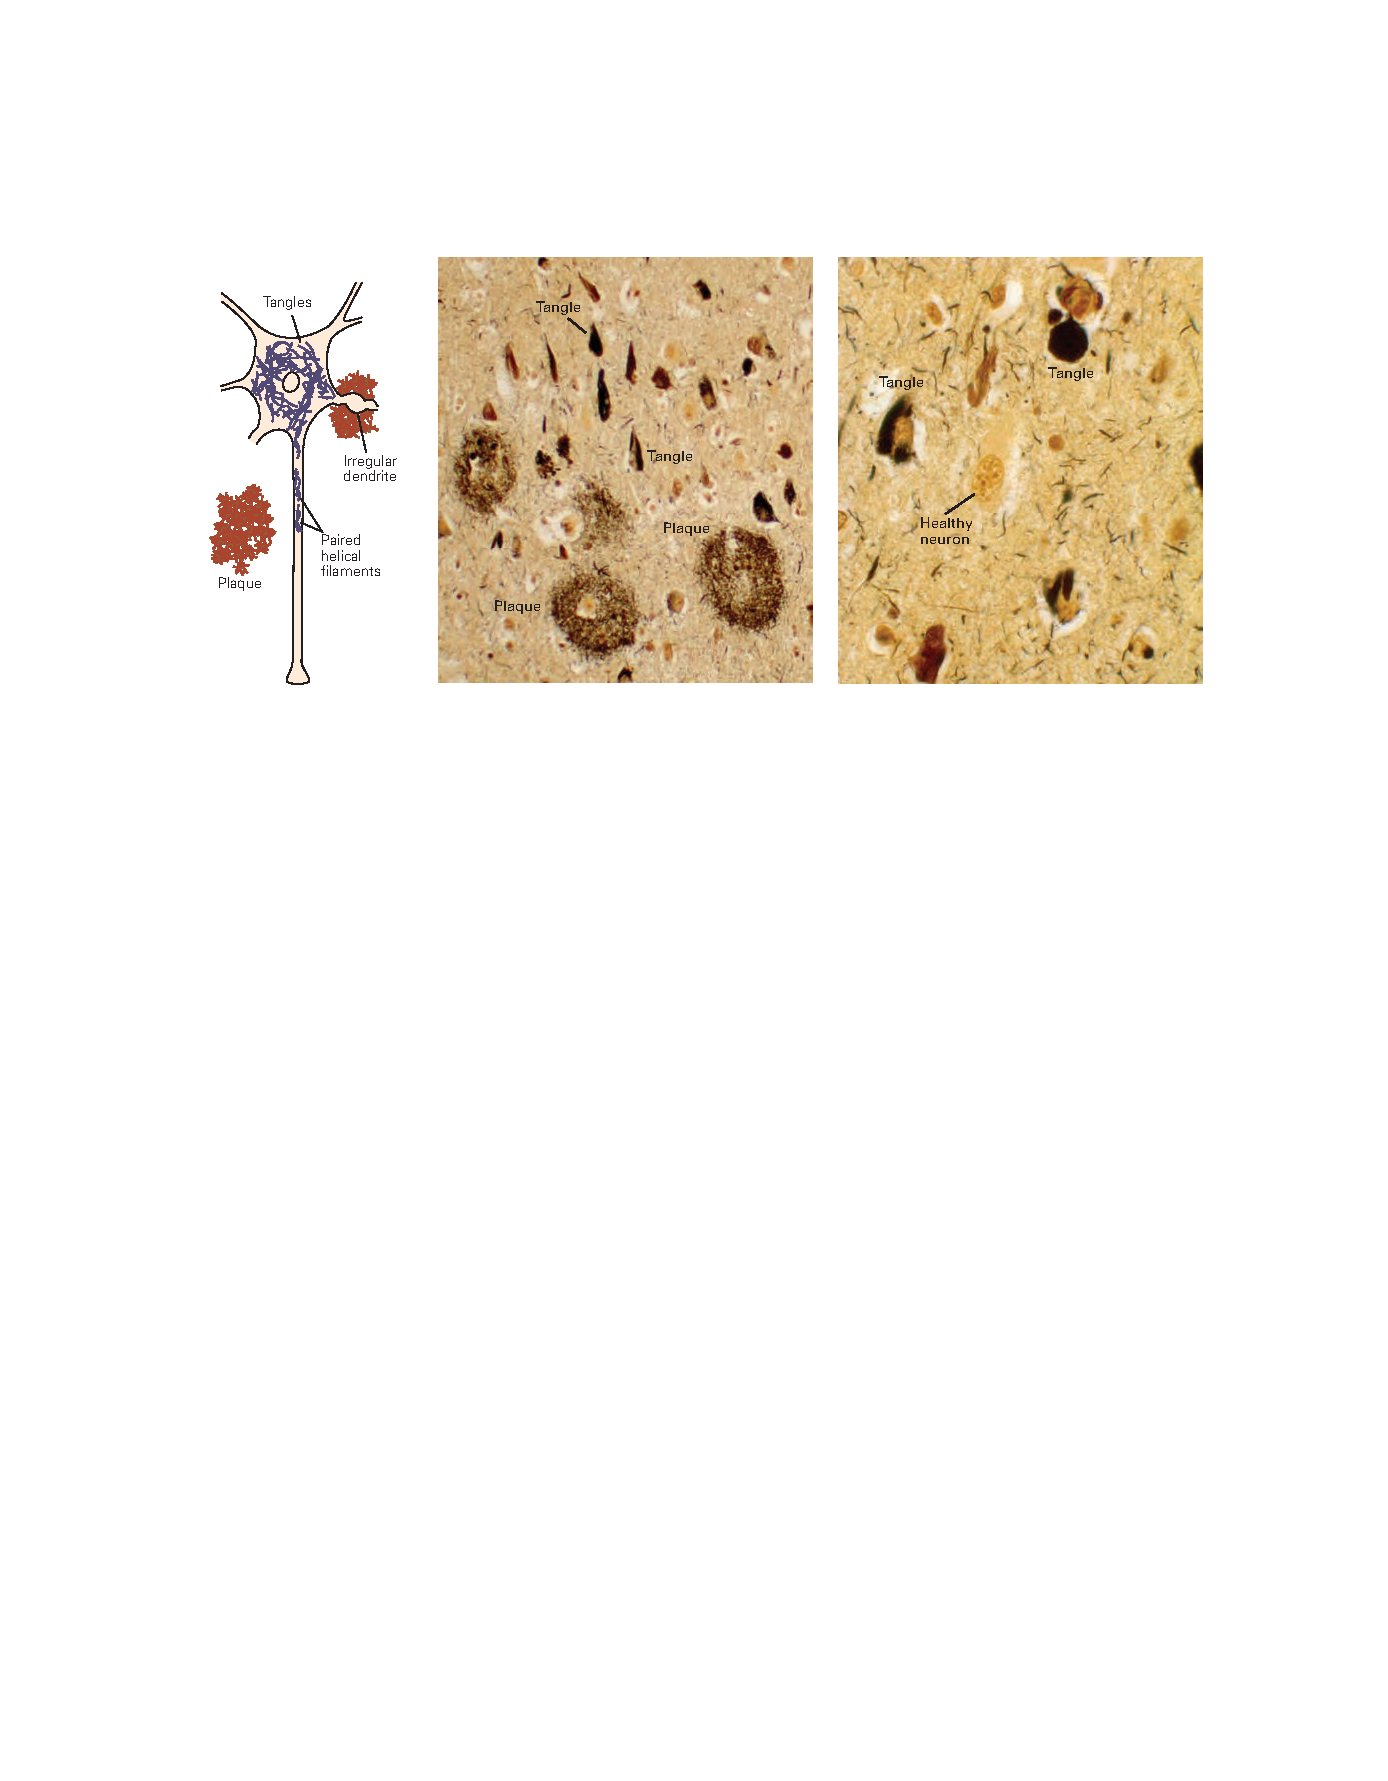
\includegraphics[width=0.9\linewidth]{chap64/fig_64_9}
	\caption{阿尔茨海默病大脑中的斑块和缠结。 患有严重阿尔茨海默病的人的大脑皮层部分显示出特征性斑块和神经原纤维缠结。 (图片经 James Goldman 许可转载。)左图:该图显示了一个神经元,其细胞体和轴突中含有神经原纤维缠结。 淀粉样斑块显示在神经细胞中; 其中一个围绕着一个树突,树突显示出一种改变的、肿胀的形状。 缠结由成对的螺旋丝束组成,由过度磷酸化的 tau 蛋白的异常聚合物组成,而淀粉样斑块是淀粉样蛋白-β (A4) 肽聚合物的细胞外沉积物。 中图:阿尔茨海默病患者的新皮层部分经银染处理后显示含有神经原纤维缠结的神经元细胞体和含有淀粉样蛋白斑块的神经细胞。 右:皮质的更高放大倍数显示神经元细胞体中的神经原纤维缠结和没有缠结的健康神经元。 在 neuropil 中可以看到许多薄的银阳性细胞突起。}
	\label{fig:64_9}
\end{figure}


第三,许多受到阿尔茨海默病病理学影响但仍然存活的神经元具有细胞骨架异常,其中最显着的是神经原纤维缠结和神经纤维丝的积累(图 \ref{fig:64_9})。
缠结是细胞体和树突中的丝状内含物,包含成对的螺旋丝和 15 纳米直丝。
这些细丝由正常微管相关蛋白 tau 的聚集形式组成。


在 AD 中,缠结不会在整个大脑中均匀发生,而是会影响特定区域。
内嗅皮质、海马体、部分新皮质和基底核特别脆弱(图 \ref{fig:64_10})。
内嗅皮质和海马体的改变可能是情景记忆问题的基础,而情景记忆是 AD 的首发症状之一。
基底前脑胆碱能系统的异常可能导致认知困难和注意力缺陷。
这些胆碱能异常与额纹状体回路中的异常形成对比,后者与正常受试者的年龄相关认知能力下降相关。
解剖差异、病理变化、广泛的神经元死亡和基因突变(见下文)的结合反对曾经流行的观点,即 AD 是正常衰老过程的异常形式。


\begin{figure}[htbp]
	\centering
	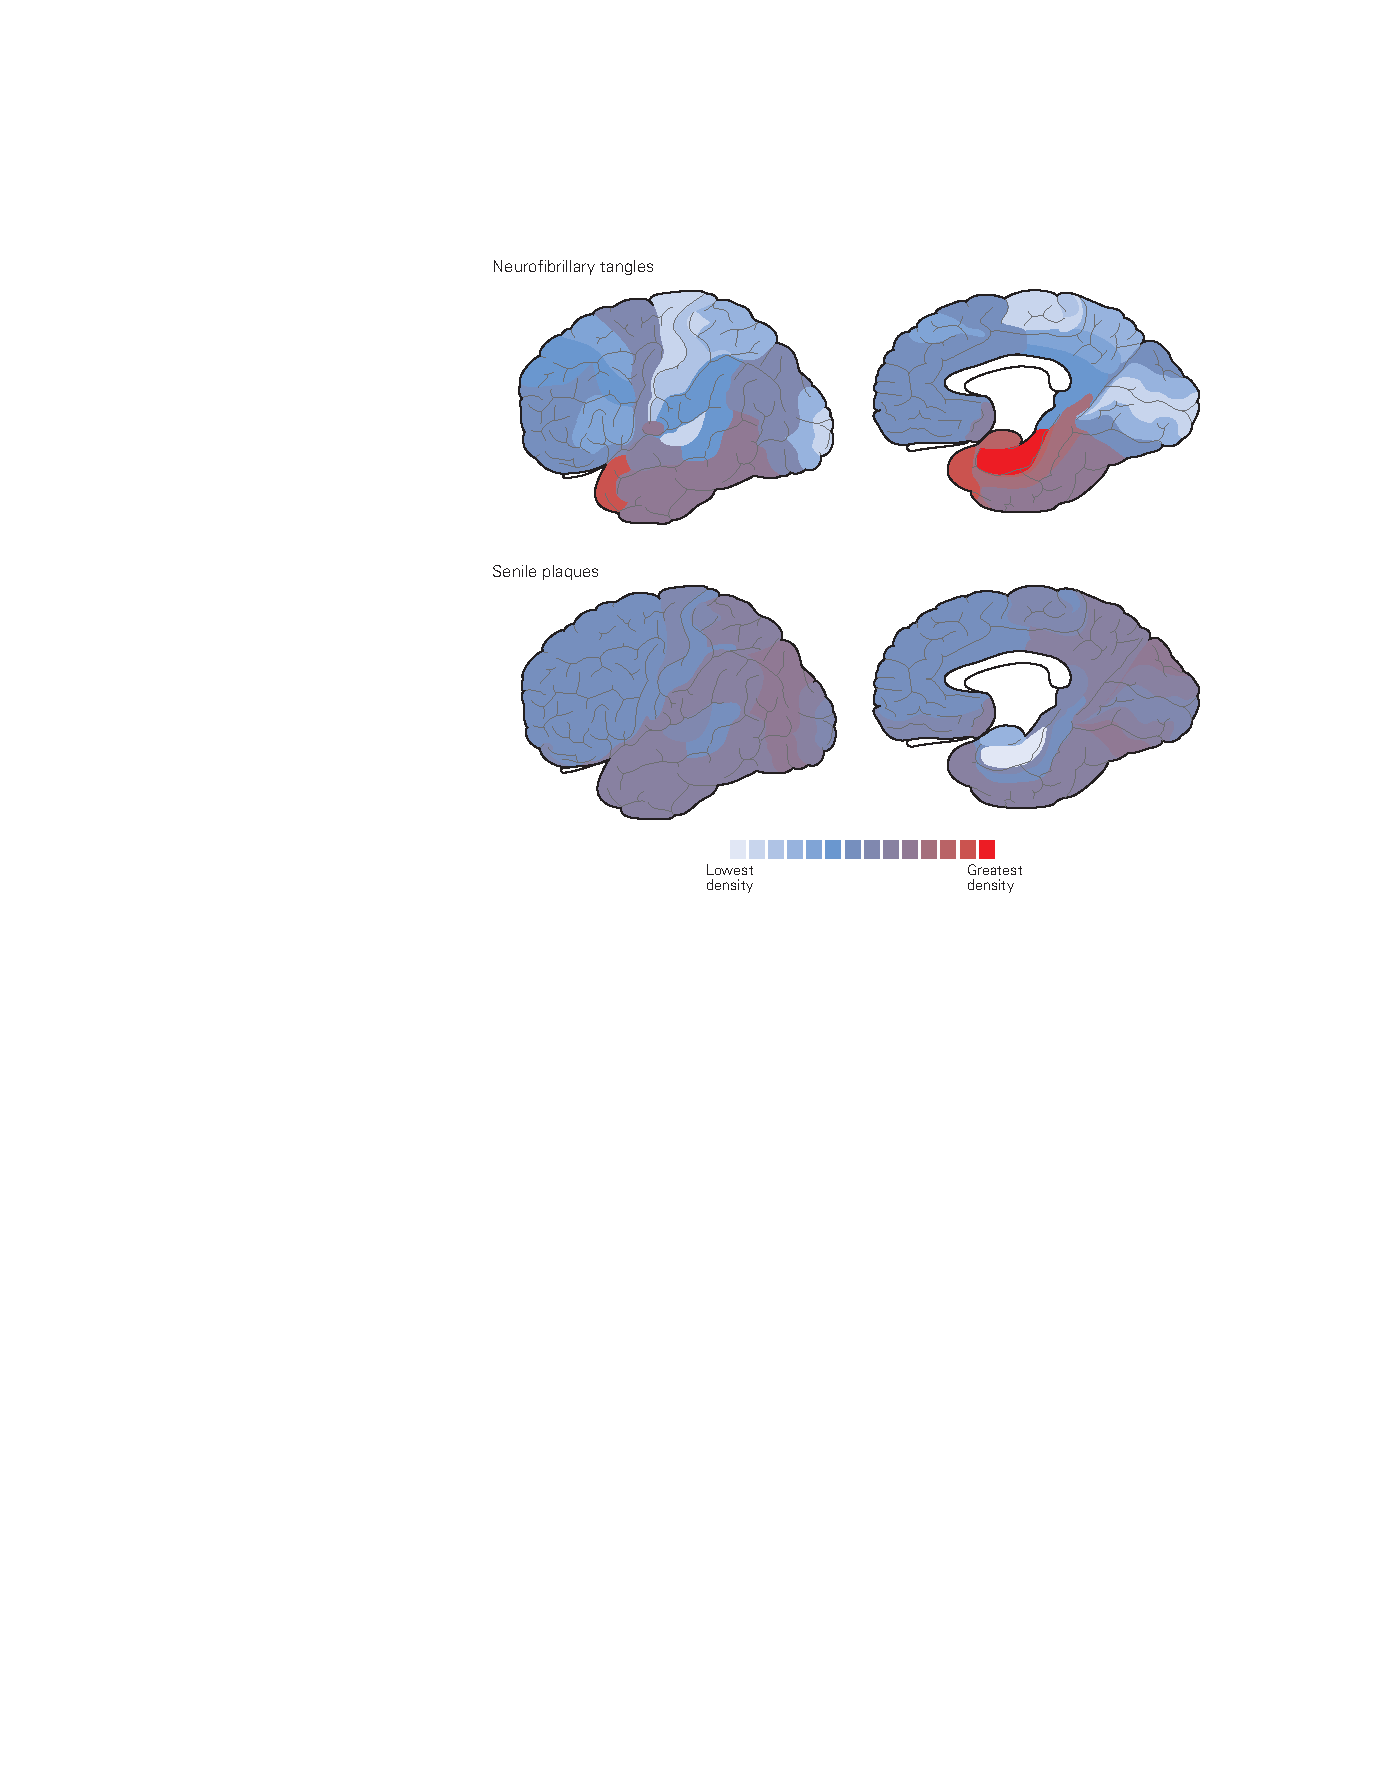
\includegraphics[width=0.7\linewidth]{chap64/fig_64_10}
	\caption{神经原纤维缠结和老年斑集中在阿尔茨海默病大脑的不同区域。 (经许可改编自 Arnold 等人,1991 年。版权所有 © 1991,牛津大学出版社。)}
	\label{fig:64_10}
\end{figure}



\subsection{淀粉样斑块含有有助于阿尔茨海默病病理学的有毒肽}

淀粉样斑块的主要成分,即 Aβ 肽的聚集体,基于其低溶解度,于 1980 年代初首次通过离心分离。
主要肽的长度为 40 和 42 个氨基酸(40 个残基加上羧基末端的两个额外氨基酸)。
生化研究表明,Aβ42 肽比 Aβ40 更快地成核成淀粉样原纤维。


相当多的实验证据表明,Aβ42 驱动初始聚集,尽管 Aβ40 也在显着程度上积累,尤其是在脑淀粉样血管病中。
对于培养的神经元,比单体大的 Aβ42 肽形式通常比 Aβ40 的聚集形式毒性更大。
这些结果暗示 Aβ42 是淀粉样蛋白形成和 Aβ 毒性的关键驱动因素。


一旦发现长度为 38 至 43 个氨基酸的 Aβ 肽是由前体蛋白的裂解形成的,研究人员便着手分离前体。
该前体于 20 世纪 80 年代中期被发现,经过分子克隆,并命名为淀粉样前体蛋白 (APP)。
它是一种大型跨膜糖蛋白,存在于所有类型的细胞中,但在神经元中以最高水平表达。
APP在大脑中的正常功能尚不清楚。


APP是如何加工形成Aβ肽的?
结果证明答案很复杂。
α-、β-和 γ-分泌酶这三种酶将 APP 切成碎片。
β- 和 γ- 分泌酶裂解 APP 产生可溶性细胞外片段,释放到间质液中。
这些是 Aβ 肽,包括 APP 的跨膜部分(图 \ref{fig:64_11})。
γ-分泌酶的切割是不寻常的,因为它发生在 APP 的跨膜部分,该区域长期以来被认为不受水解影响,因为它被脂质而不是水包围。
在 Aβ 序列中间被 α-分泌酶切割可防止 Aβ 肽的形成。


\begin{figure}[htbp]
	\centering
	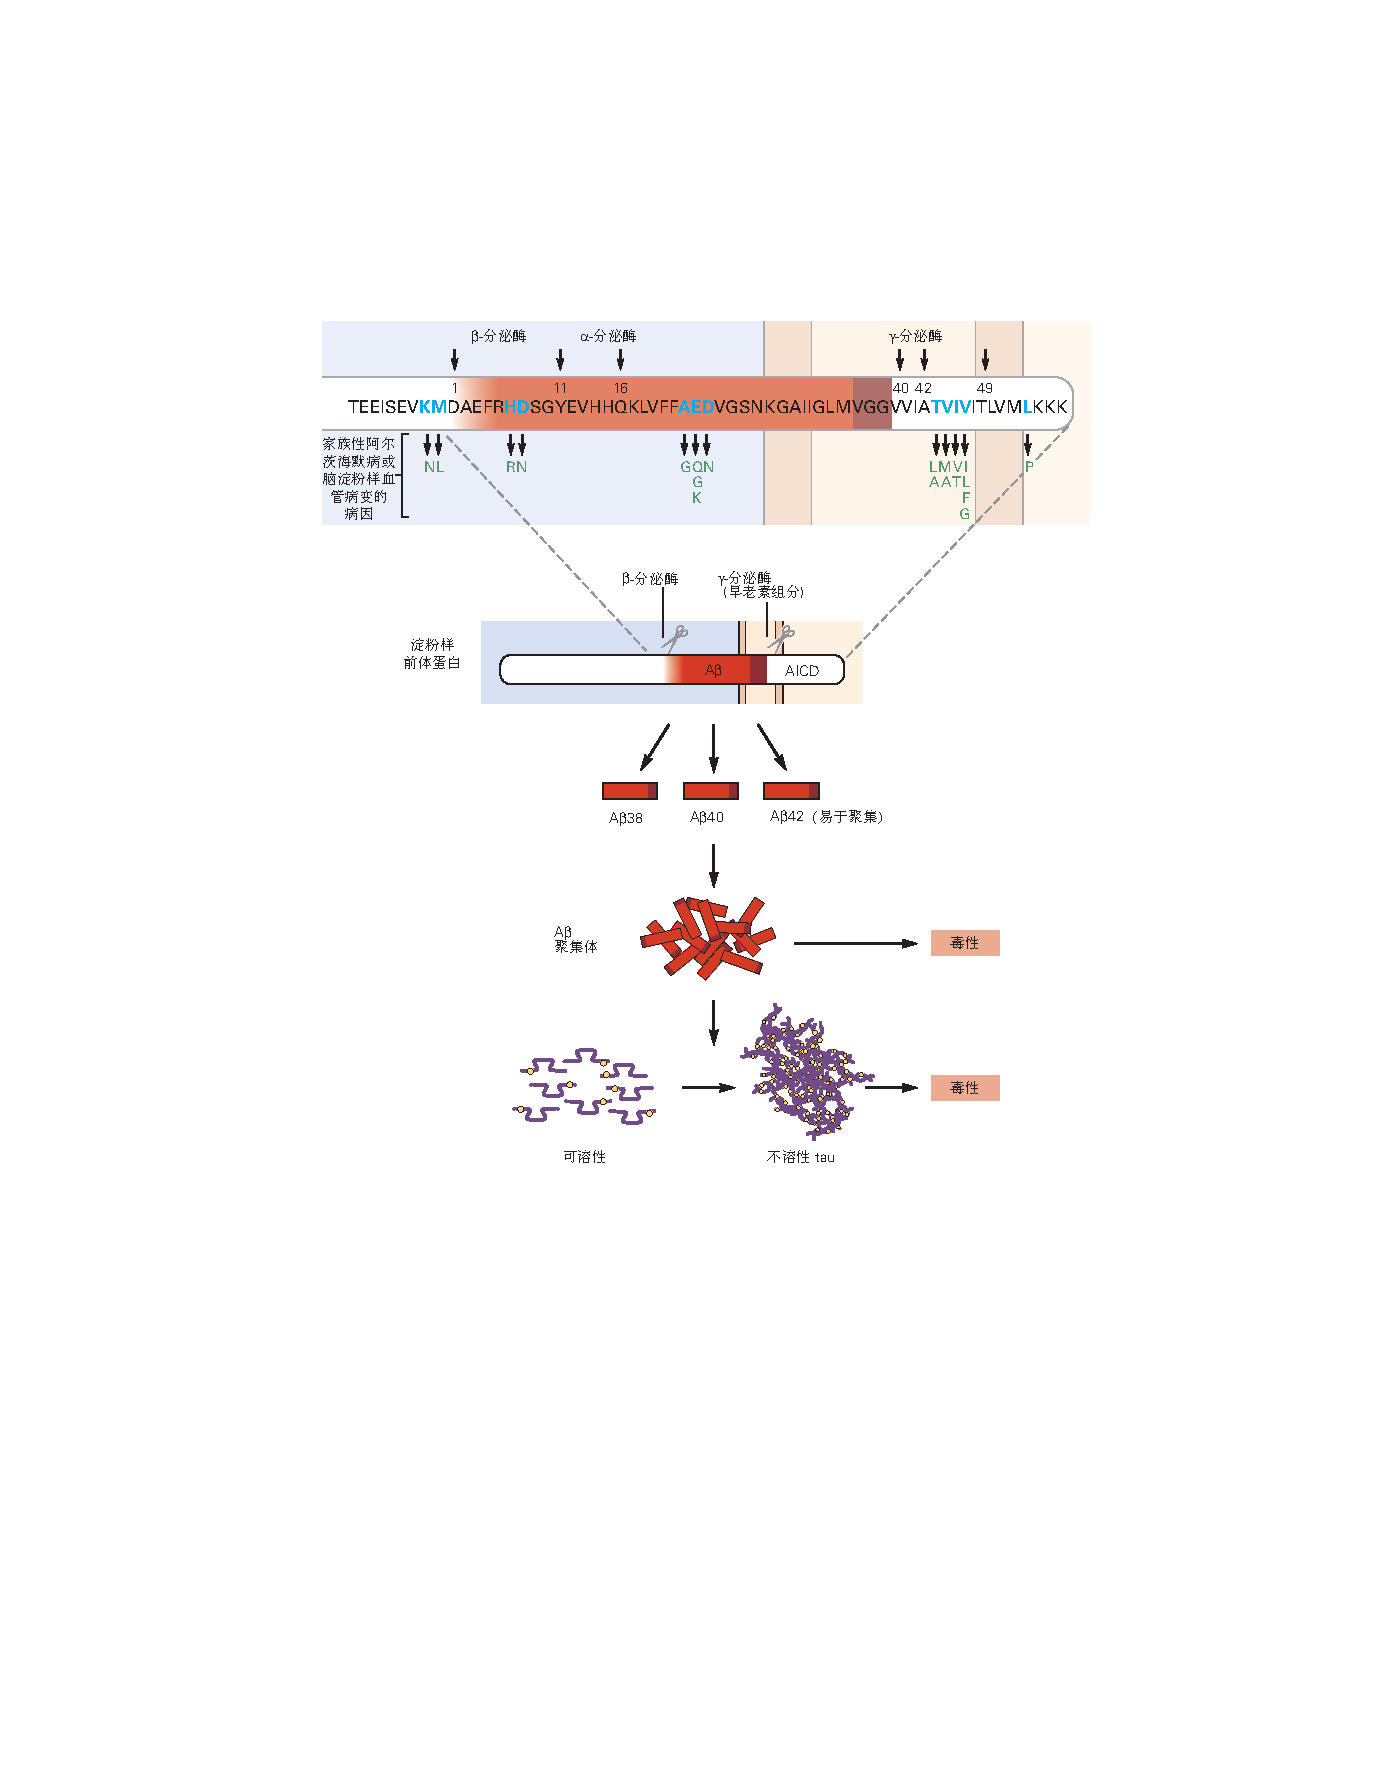
\includegraphics[width=0.8\linewidth]{chap64/fig_64_11}
	\caption{淀粉样蛋白前体蛋白的加工、Aβ 肽的产生以及对 tau 聚集的下游影响。 Aβ 肽是由淀粉样蛋白前体蛋白 (APP)(一种跨膜蛋白)通过两种酶(β-分泌酶和 γ-分泌酶)裂解产生的。 (α-分泌酶的切割可防止 Aβ 的产生。)早老素是 γ-分泌酶复合物的活性酶促成分,可在膜内的多个位点切割 APP 以产生不同长度的 Aβ 肽,例如 Aβ38、Aβ40 和 Aβ42。 APP 中位于 Aβ 区域之外或 Aβ 编码序列内的几种突变会导致常染色体显性阿尔茨海默病 (AD) 的形式。 APP/Aβ氨基酸序列中的氨基酸(蓝色)代表APP中的正常氨基酸; 绿色氨基酸(低于正常序列)是导致家族性 AD 或脑淀粉样血管病 (CAA) 的氨基酸。 Aβ 主要由核内体内的 APP 产生。 多种分子和突触活动调节 Aβ 水平。 有证据表明 Aβ 聚集受 Aβ 结合分子 ApoE 和凝聚素的影响,它们可能在大脑的细胞外空间相互作用。 多种分子和过程影响 Aβ 从存在于大脑细胞外空间的间质液 (ISF) 中清除,包括脑啡肽酶和胰岛素降解酶 (IDE),以及脑脊髓液和间质液体积流量。 LRP1 和 RAGE(晚期糖基化终产物的受体)似乎影响 Aβ 穿过血脑屏障的转运。 Aβ 的浓度和类型会影响聚集(Aβ42 更易形成纤维)。 一旦它聚集成低聚物和原纤维,它就会对细胞产生直接毒性,诱发炎症,并通过尚不清楚的机制加剧可溶性 tau 向聚集 tau 的转化。 除 Aβ 外,还有多种因素影响 tau 聚集和毒性,包括 tau 水平、序列和磷酸化状态。 (缩写:AICD,APP胞内结构域。)}
	\label{fig:64_11}
\end{figure}


已经分离和表征了负责 α-、β- 和 γ- 分泌酶的酶。
α-分泌酶是称为 ADAM(一种解联蛋白和金属蛋白酶)的细胞外蛋白酶大家族的成员,负责降解细胞外基质的许多成分。
β-分泌酶,称为 BACE1(β-位点 APP 裂解酶 1),是中枢神经元中的一种跨膜蛋白,集中在突触中。
来自缺乏 BACE1 的突变小鼠的脑细胞不产生 Aβ 肽,证明 BACE1 确实是神经元 β-分泌酶。
γ-分泌酶是三者中最复杂的,实际上是一种多蛋白复合物,可以切割几种不同的跨膜蛋白。
正如预期的那样,鉴于其在膜内发挥作用的特殊能力,γ-分泌酶本身包括几种跨膜蛋白。
其中两个称为早老素 1 和早老素 2,反映了它们与 AD 的关联。
该复合物的其他成分包括跨膜蛋白 nicastrin、Aph-1 和 Pen-2。


尽管 Aβ 和 APP 的生化特性很有趣,但关键问题是它们是否参与了 AD 的衰弱症状。
该疾病可能是由 Aβ 积累引起的,但 Aβ 本身可能是另一种病理过程的结果,甚至是无害的相关因素。
人类和实验动物的遗传证据对于证明 APP,特别是 Aβ 在 AD 中发挥核心作用至关重要。


第一条线索来自对 APP 基因位于 21 号染色体上的观察,唐氏综合症患者(也称为 21 三体综合征)中存在三个拷贝,而不是正常的两个拷贝。
所有活到中年的唐氏综合症患者都会在 50 岁左右出现 AD 病理和痴呆症。
这种关联与 APP 通过在整个生命过程中过量产生 APP 和 Aβ 50\% 来诱发 AD 的观点是一致的。
然而,许多基因的拷贝在 21 三体个体中以三个拷贝存在,最初,尚不清楚唐氏综合症中 APP 的三倍体是导致该人群 AD 的原因。
随后,由于人类 21 号染色体上 APP 基因座的重复,发现了在没有唐氏综合症的情况下同时发生 AD 和脑淀粉样血管病的罕见家族。
这是强有力的证据表明,仅 APP 的过度表达就足以导致 AD 和 脑淀粉样血管病。


更直接的遗传证据来自对罕见的显性遗传性 AD 患者的分析,这些患者的症状发作通常在 30 至 50 岁之间。
在 20 世纪 80 年代后期,几个研究小组开始使用分子克隆方法来鉴定在显性遗传 AD 中发生突变的基因。
值得注意的是,识别出的前三个基因是编码蛋白质 APP、presenilin-1 和 presenilin-2 的基因(图 \ref{fig:64_12})。
在这三个基因中发现了许多不同的突变,大多数影响 APP 的切割,增加 Aβ 肽的产生,或者特别是更容易聚集的 Aβ42 物种的比例。
有趣的是,一些 APP 突变发生在 Aβ 序列本身内,不会影响 Aβ 的产生,但会影响 Aβ 的聚集和从大脑中清除。


\begin{figure}[htbp]
	\centering
	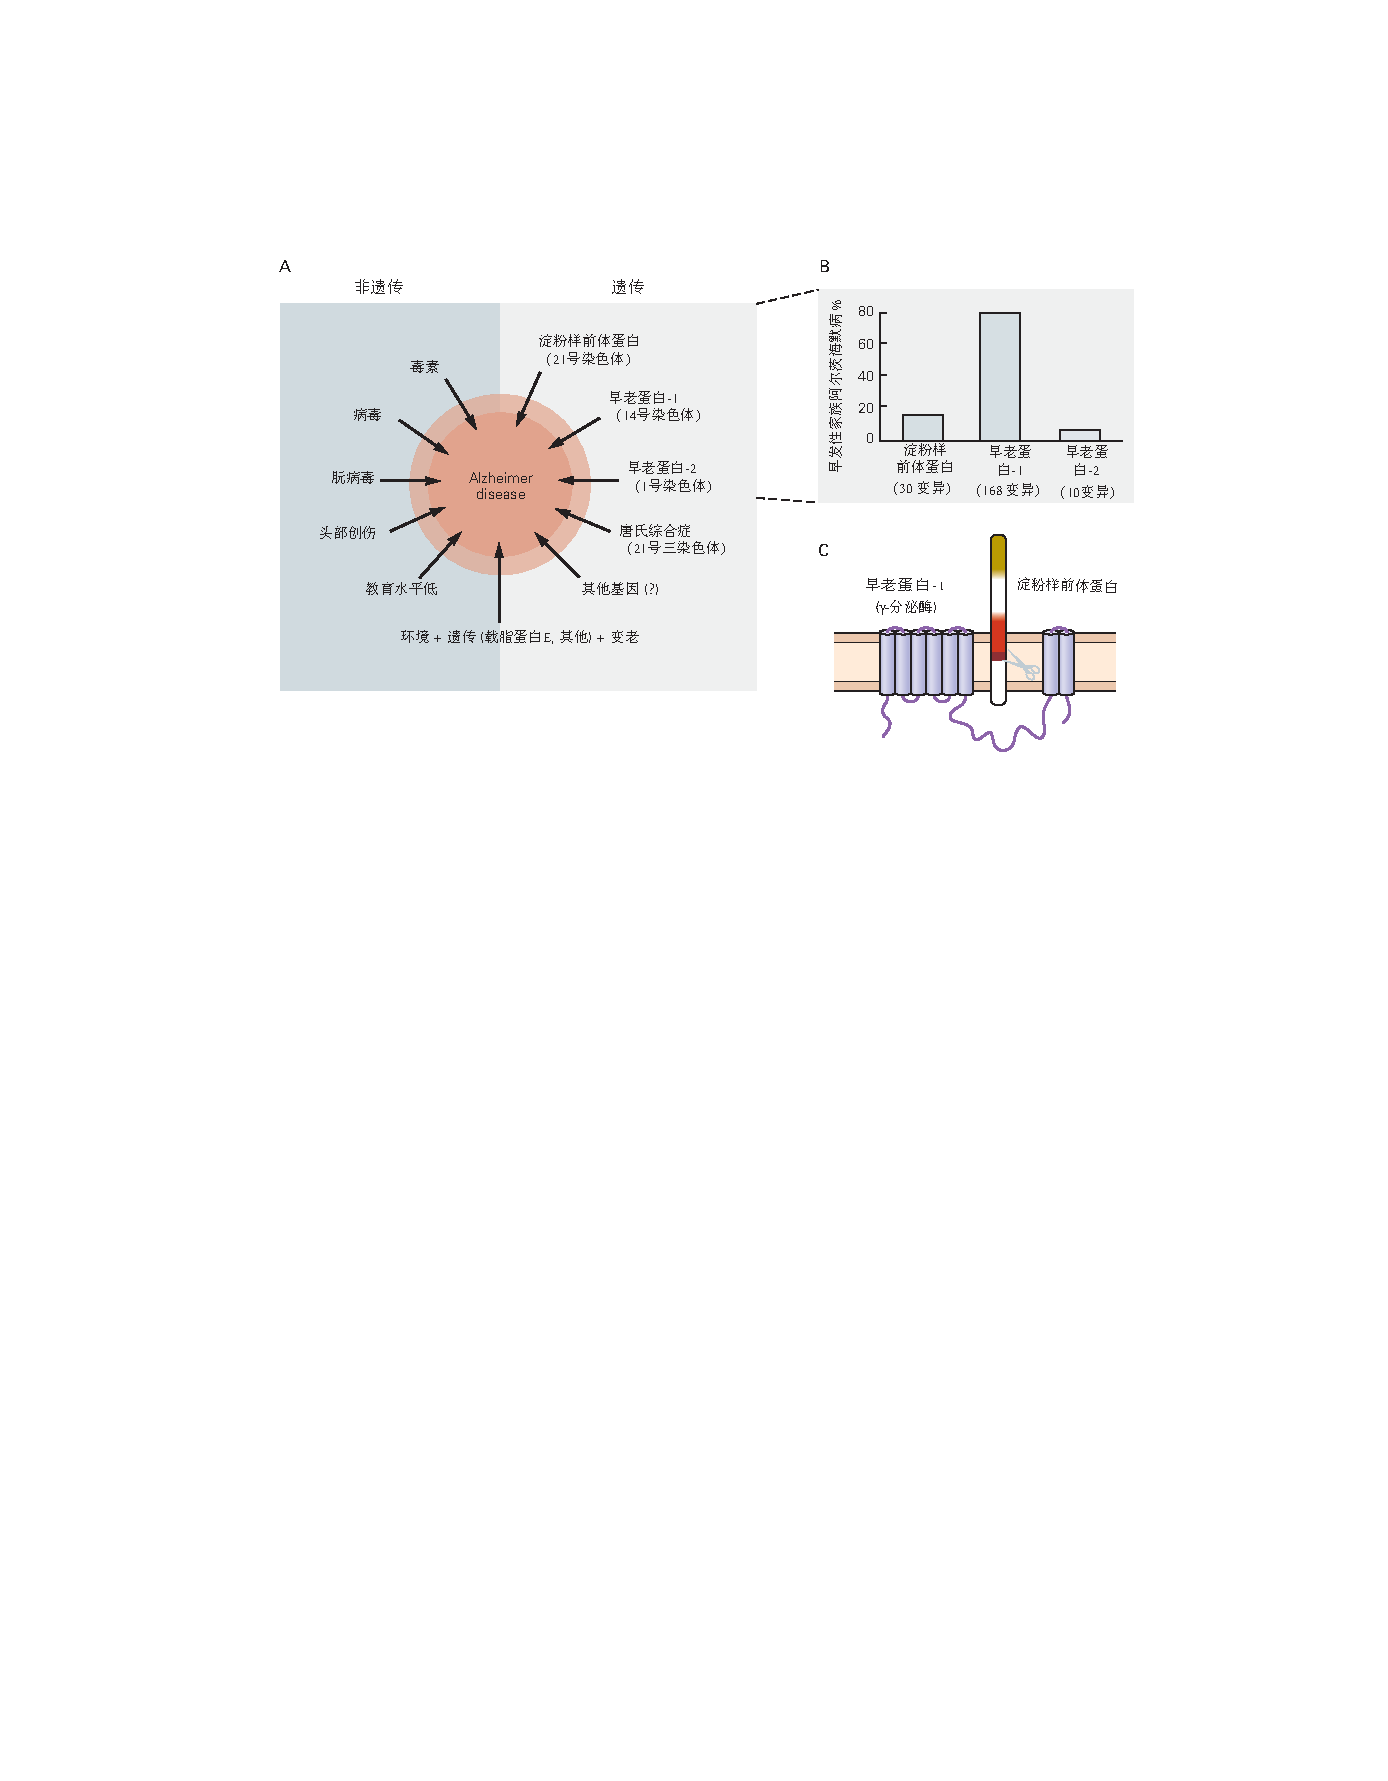
\includegraphics[width=0.8\linewidth]{chap64/fig_64_12}
	\caption{环境和遗传因素在阿尔茨海默病中发挥作用。 A. 环境和遗传因素。 (缩写:APOE,载脂蛋白 E;APP,淀粉样前体蛋白;PS1,presenilin-1;PS2,presenilin-2。)B. 早发性阿尔茨海默病 (AD) 中涉及的特定基因。 C. Presenilin-1(γ 分泌酶复合物的一种成分)与质膜内的 APP 蛋白相关。}
	\label{fig:64_12}
\end{figure}


一些 APP 突变是 Aβ 区域两侧的氨基酸置换。
在 β-分泌酶切割位点表达双重突变的细胞(所谓的瑞典突变)是 Aβ 形成所必需的,其分泌的 Aβ 肽比表达野生型 APP 的细胞多几倍。
有趣的是,最近发现了与 β-分泌酶位点相邻的 APP 中的另一个突变。
这种突变似乎通过减少 Aβ 的产生来预防 AD。 另一个 APP 突变导致 γ-分泌酶产生更大比例的较长 Aβ 种类,例如 Aβ42,相对于较短的种类,例如 Aβ40。
同样,在大多数早老素突变体中,突变体 γ-分泌酶的活性高于正常水平或产生 Aβ42 与 Aβ40 比例增加的肽。


这些人类遗传学研究提供了令人信服的证据,证明 (1) APP 裂解产生 Aβ 和 Aβ 聚集的倾向在某些显性遗传的早发性 AD 病例中起着关键的促进作用,以及 (2) 较少的 Aβ 产生降低了晚发的风险 广告。
小鼠遗传学研究也加强了 APP 切割,特别是 Aβ 聚集导致 AD 的情况。
转基因表达或敲入与常染色体显性遗传 AD 中发现的相同的突变 APP 形式导致海马和皮质中出现淀粉样蛋白斑块、Aβ 沉积物附近的营养不良神经突、淀粉样蛋白斑块周围突触末端密度降低和损伤 在突触传递中。
一些小鼠模型出现功能异常,例如空间和情景记忆缺陷。
在表达改变形式的 APP 和早老素-1 的转基因小鼠中,改变更为严重。
重要的是要注意,尽管这些小鼠不会出现 tau 聚集或神经原纤维缠结,这些病变被认为在 AD 中的认知能力下降中很重要,但它们仍然是解决 Aβ 的机制作用和 AD 发病机制中相关病理学的宝贵模型 ,尤其是 Aβ 的作用,以及用于测试潜在疗法。


鉴于 APP 裂解参与 AD 发病机制的有力证据,下一个问题是:
裂解产物的积累如何导致症状并最终导致痴呆? 存在三组切割产物:分泌的细胞外区域(胞外域)、Aβ 肽和细胞质片段。
尽管所有这三个片段都可能对实验动物的神经元产生有害影响,但 Aβ 肽受到的关注最多,而且其参与的证据也是最有力的。
有证据表明,Aβ 的不同聚集形式(例如低聚物、原纤维和原纤维)可导致可能导致 AD 的突触和神经元损伤。



\subsection{神经原纤维缠结含有微管相关蛋白}
直到 2005 年左右,大多数关于 AD 分子和细胞基础的研究都集中在 Aβ 肽和淀粉样斑块上,但神经原纤维缠结中的 tau 聚集似乎在 AD 的进展中起着关键作用(图 \ref{fig:64_9})。
分子分析表明,细胞体和近端树突中的这些异常内含物含有过度磷酸化的 tau 异构体的聚集体,tau 是一种通常可溶的微管结合蛋白(图 \ref{fig:64_13})。
tau 蛋白通过结合并稳定微管,在细胞内运输中发挥关键作用,尤其是在轴突中。
轴突运输受损会损害突触稳定性和营养支持。
虽然 tau 蛋白的聚集和过度磷酸化导致毒性的机制尚不清楚,但 tau 蛋白的积累显然与神经元变性有关。


\begin{figure}[htbp]
	\centering
	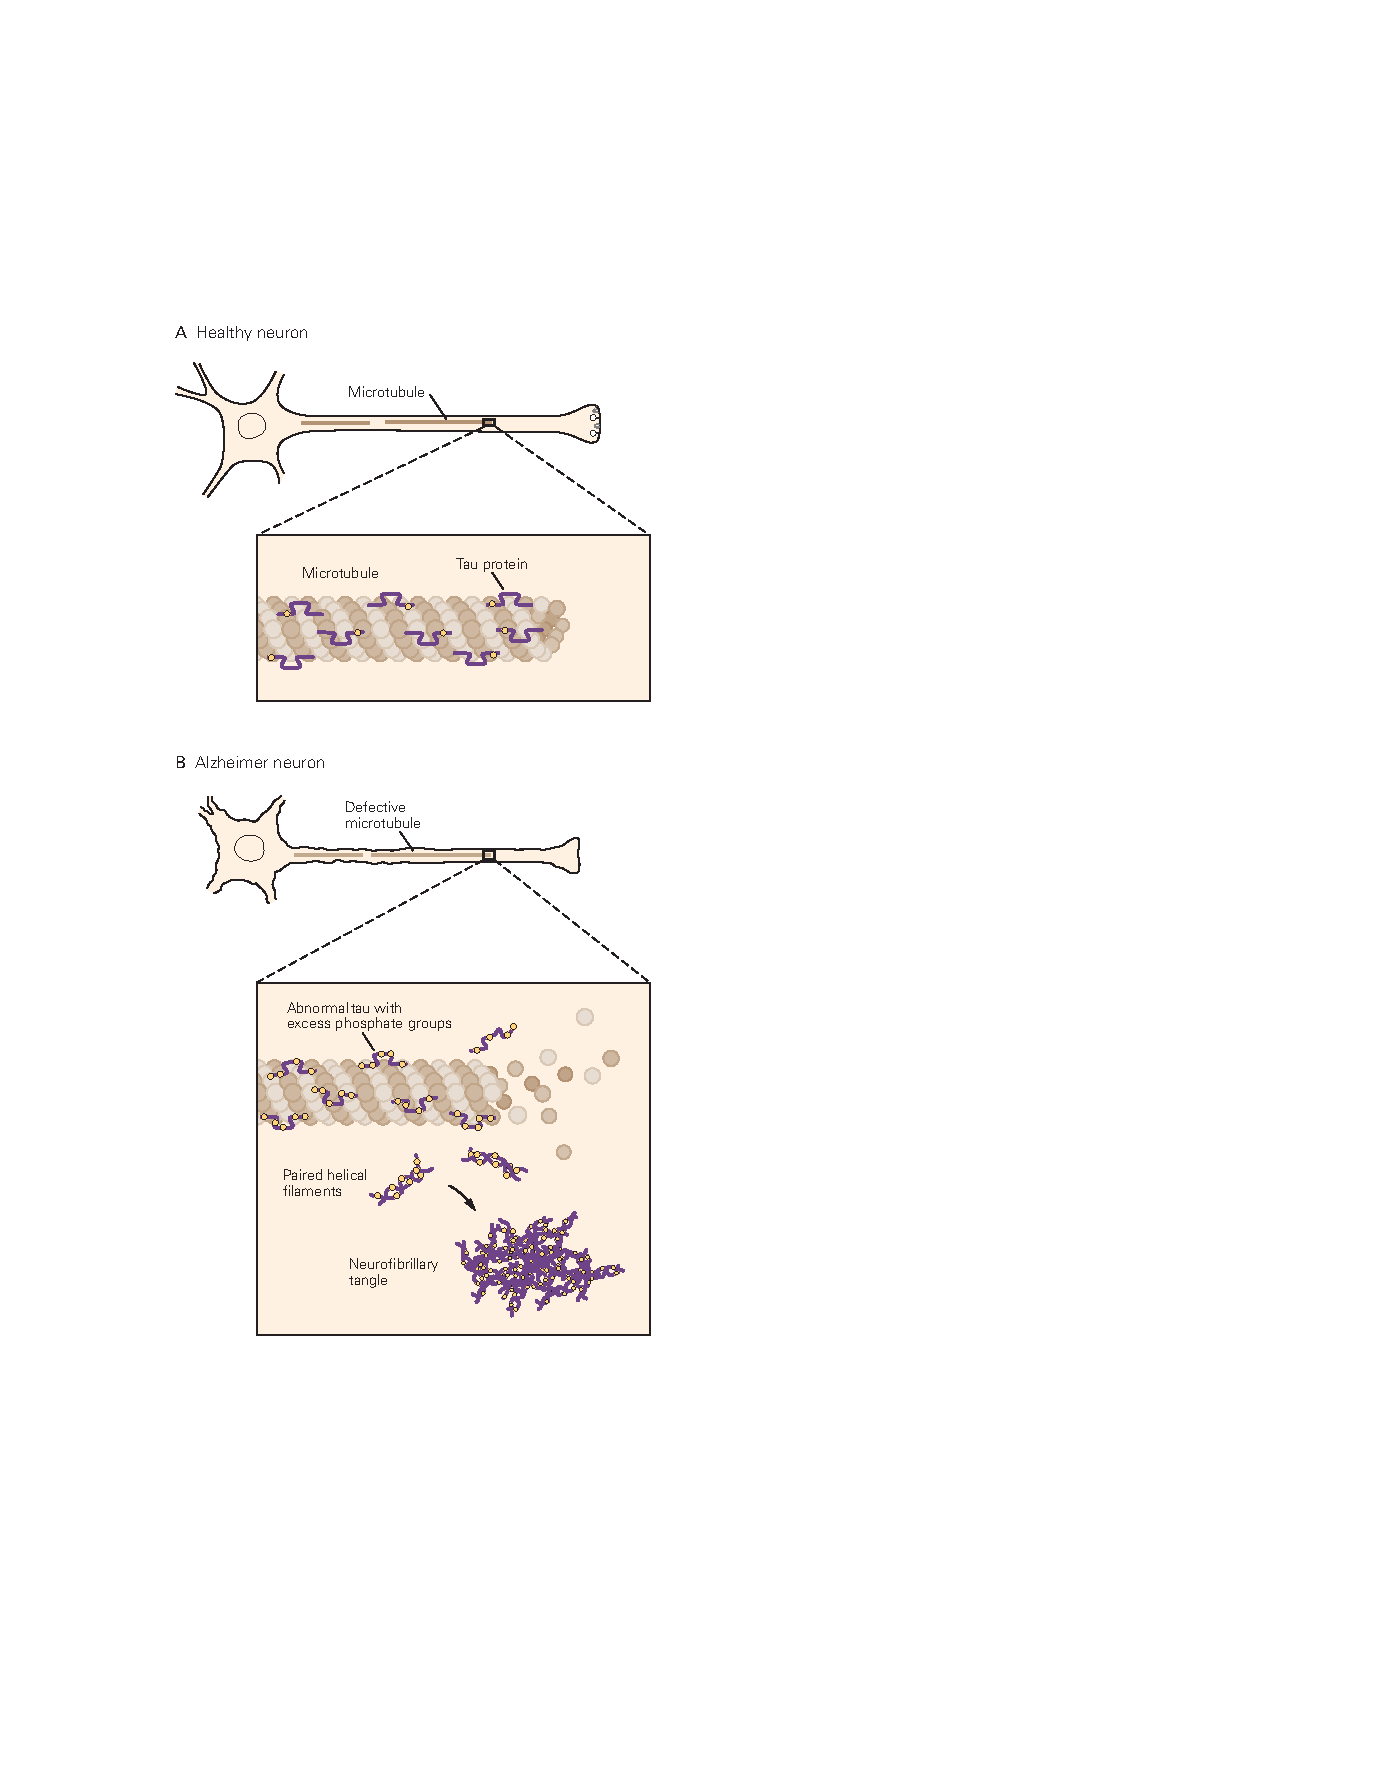
\includegraphics[width=0.5\linewidth]{chap64/fig_64_13}
	\caption{神经原纤维缠结的形成。 A. 在健康的神经元中,tau 蛋白与正常的微管结合但不是成对的螺旋丝,并有助于神经元的结构完整性。 B. 在患病的神经元中,tau 蛋白变得过度磷酸化并失去与开始分解的正常微管的联系。 然后它形成成对的螺旋丝,被隔离在神经原纤维缠结中。}
	\label{fig:64_13}
\end{figure}


尽管缠结是 AD 的一个决定性特征,但最初并不清楚缠结和过度磷酸化形式的 tau 在疾病的发病机制中扮演什么角色。
虽然 APP 和早老素基因的突变可导致 AD,但在家族性 AD 中未发现 tau 基因的突变。
然而,现在有大量证据表明 tau 聚集是 AD 中发生的神经变性的关键因素。


首先,在多种神经退行性疾病中都可以看到过度磷酸化 tau 的丝状沉积物,包括 AD、各种形式的额颞叶痴呆、进行性核上性麻痹、皮质基底节变性和 CTE。
其次,已发现 tau 基因突变是另一种常染色体显性神经退行性疾病形式的基础:帕金森病 17 型额颞叶痴呆 (FTPD17)。
在没有 Aβ 沉积的情况下,这些患者在特定脑区发生 tau 聚集和脑萎缩。
第三,AD 的进行性症状与缠结的数量和分布的相关性要好于与尸检中观察到的淀粉样蛋白斑块的相关性。
例如,在该区域出现斑块之前,缠结通常首先在内嗅皮层和海马体(早期记忆障碍的可能部位)的神经元中出现(见图 \ref{fig:64_16})。


\begin{figure}[htbp]
	\centering
	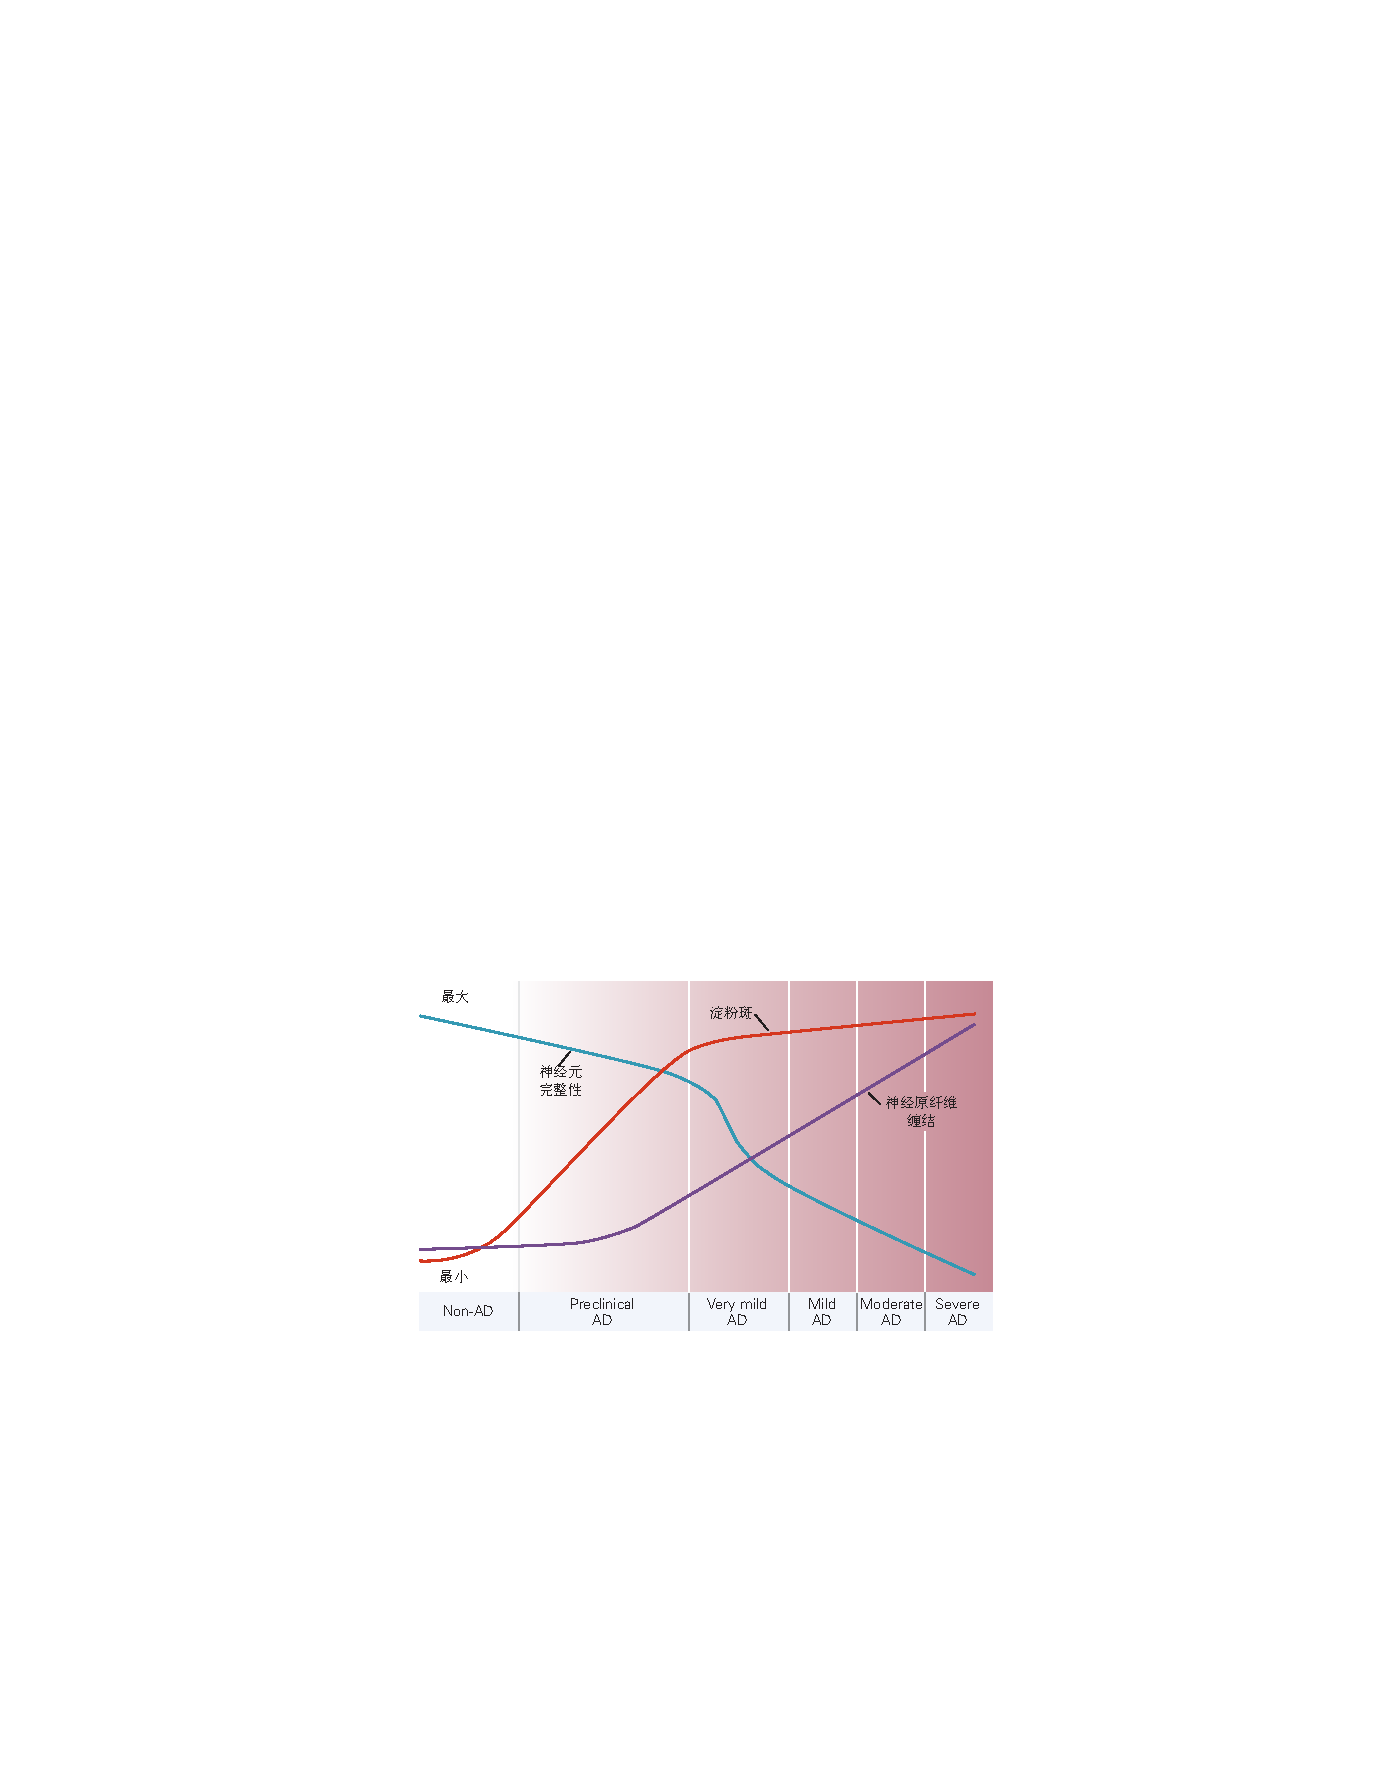
\includegraphics[width=0.7\linewidth]{chap64/fig_64_16}
	\caption{生物标志物变化与阿尔茨海默病 (AD) 认知和临床变化的关系。 在将要发展为 AD 痴呆症的认知正常人群中,最初的体征之一是 Aβ 以淀粉样蛋白斑块的形式在大脑中开始聚集。 虽然人们的认知能力仍然正常,但淀粉样斑块会继续积累。 在某个时候,大约在任何明显的认知衰退发生前 5 年,tau 蛋白在新皮质中的积累开始增加,炎症和氧化应激增加,大脑网络连接和新陈代谢开始下降。 神经元和突触丢失以及脑萎缩也开始了。 这个时期——当患者保持认知正常但 AD 型病理正在形成时——被称为临床前 AD。 一旦有足够的神经元和突触功能障碍以及细胞丢失,就会出现非常轻度的痴呆和轻度认知障碍。 那时,淀粉样蛋白沉积几乎达到顶峰。 随着痴呆症恶化到轻度、中度和重度阶段,神经原纤维缠结形成,神经元和突触功能障碍、炎症、细胞死亡和脑萎缩恶化。 (经许可改编自 Perrin、Fagan 和 Holtzman 2009。)}
	\label{fig:64_16}
\end{figure}


多年来,那些认为 Aβ 是 AD 的主要致病因子的人和那些认为富含 tau 蛋白的缠结起主要作用的人之间一直存在争议。
这些游击队员分别被称为“浸信会”和“道教”。
浸信会指出,在症状出现前约 15 年开始的 AD 病理学发展过程中,新皮质 Aβ 的积累先于新皮质 tau 病理学的发展。
然而,最近的证据表明,Aβ 的积累似乎以某种方式驱动 tau 蛋白在大脑中聚集和扩散。
因此,Aβ 聚集可能会引发疾病,而 tau 聚集和扩散可能是导致神经变性的主要方式。
例如,同时表达突变 APP 和突变 tau 的转基因小鼠会出现更严重的 tau 病理学。


斑块和缠结之间似乎存在相互作用。
将 Aβ42 注射到表达突变 tau 蛋白的转基因小鼠的特定脑区会增加附近神经元的缠结数量。
此外,减少斑块数量和大小的操作会导致过度磷酸化 tau 水平降低。
重要的是,最近的实验表明,Aβ 沉积以某种方式促进 tau 聚集体从一个大脑区域扩散到另一个大脑区域,可能以类似朊病毒的方式跨突触扩散。
这一过程的细节仍有待制定,并且可能极其重要。


现在有大量来自细胞培养和动物模型研究的证据表明,在神经退行性疾病中聚集的几种蛋白质,包括 tau 和突触核蛋白,可以以类似朊病毒的方式在细胞之间传播。
这作为一种潜在的疾病机制尤为重要。
例如,如果错误折叠蛋白质的细胞间传播发生在细胞外空间,则该过程可能会被针对适当的疾病相关蛋白质的抗体打断。
事实上,这现在已成为多项针对 tau 和突触核蛋白的人体临床试验的基础。



\subsection{已经确定了阿尔茨海默病的危险因素}

极少数个体因携带 APP 或早老素基因的常染色体显性突变等位基因而患上 AD,并且这些通常属于早发型。
几乎所有迟发性 AD 病例都是由 APP 或早老素基因突变引起的。
那么,我们可以预测这些人的 AD 吗?


主要的风险因素是年龄。
这种疾病存在于 60 岁以下的极少数人群中(其中许多是常染色体显性遗传病例),60 至 70 岁人群中的 1\% 至 3\%,70 至 80 岁人群中的 3\% 至 12\% , 以及 25\% 到 40\% 的 85 岁以上的老年人。然而,知道老年人是 AD 的主要候选人几乎没有治疗作用,因为现代医学无法减缓时间的流逝。
因此,人们对影响 AD 发病率的其他因素产生了浓厚的兴趣。


迄今为止,发现的迟发性 AD 最重要的遗传风险因素是 APOE 基因的等位基因。
ApoE 蛋白是一种载脂蛋白。
在血液中,它在血浆胆固醇代谢中起重要作用。
它也在大脑中以高水平表达,最突出的是星形胶质细胞,在一定程度上是小胶质细胞。
在大脑中,其正常功能尚未阐明,它被分泌为高密度样脂蛋白的成分。
在人类中,APOE 基因有三个等位基因,APOE2、APOE3 和 APOE4,它们之间至多相差两个氨基酸。
携带 APOE4 等位基因的人有患 AD 的风险,而携带 APOE2 等位基因的人相对于具有最常见 APOE3/APOE3 基因型的人而言可免受 AD 的侵害。
APOE4 等位基因存在于大约 25\% 的普通人群中,但存在于多达 60\% 的 AD 患者中。
相对于 ApoE3/E3 的人,一个 APOE4 等位基因拷贝增加 AD 风险约 3.7 倍,两个拷贝增加约 12 倍(图 \ref{fig:64_14})。
相对于 APOE3/APOE3,一个 APOE2 等位基因拷贝可将 AD 风险降低约 40\%。


\begin{figure}[htbp]
	\centering
	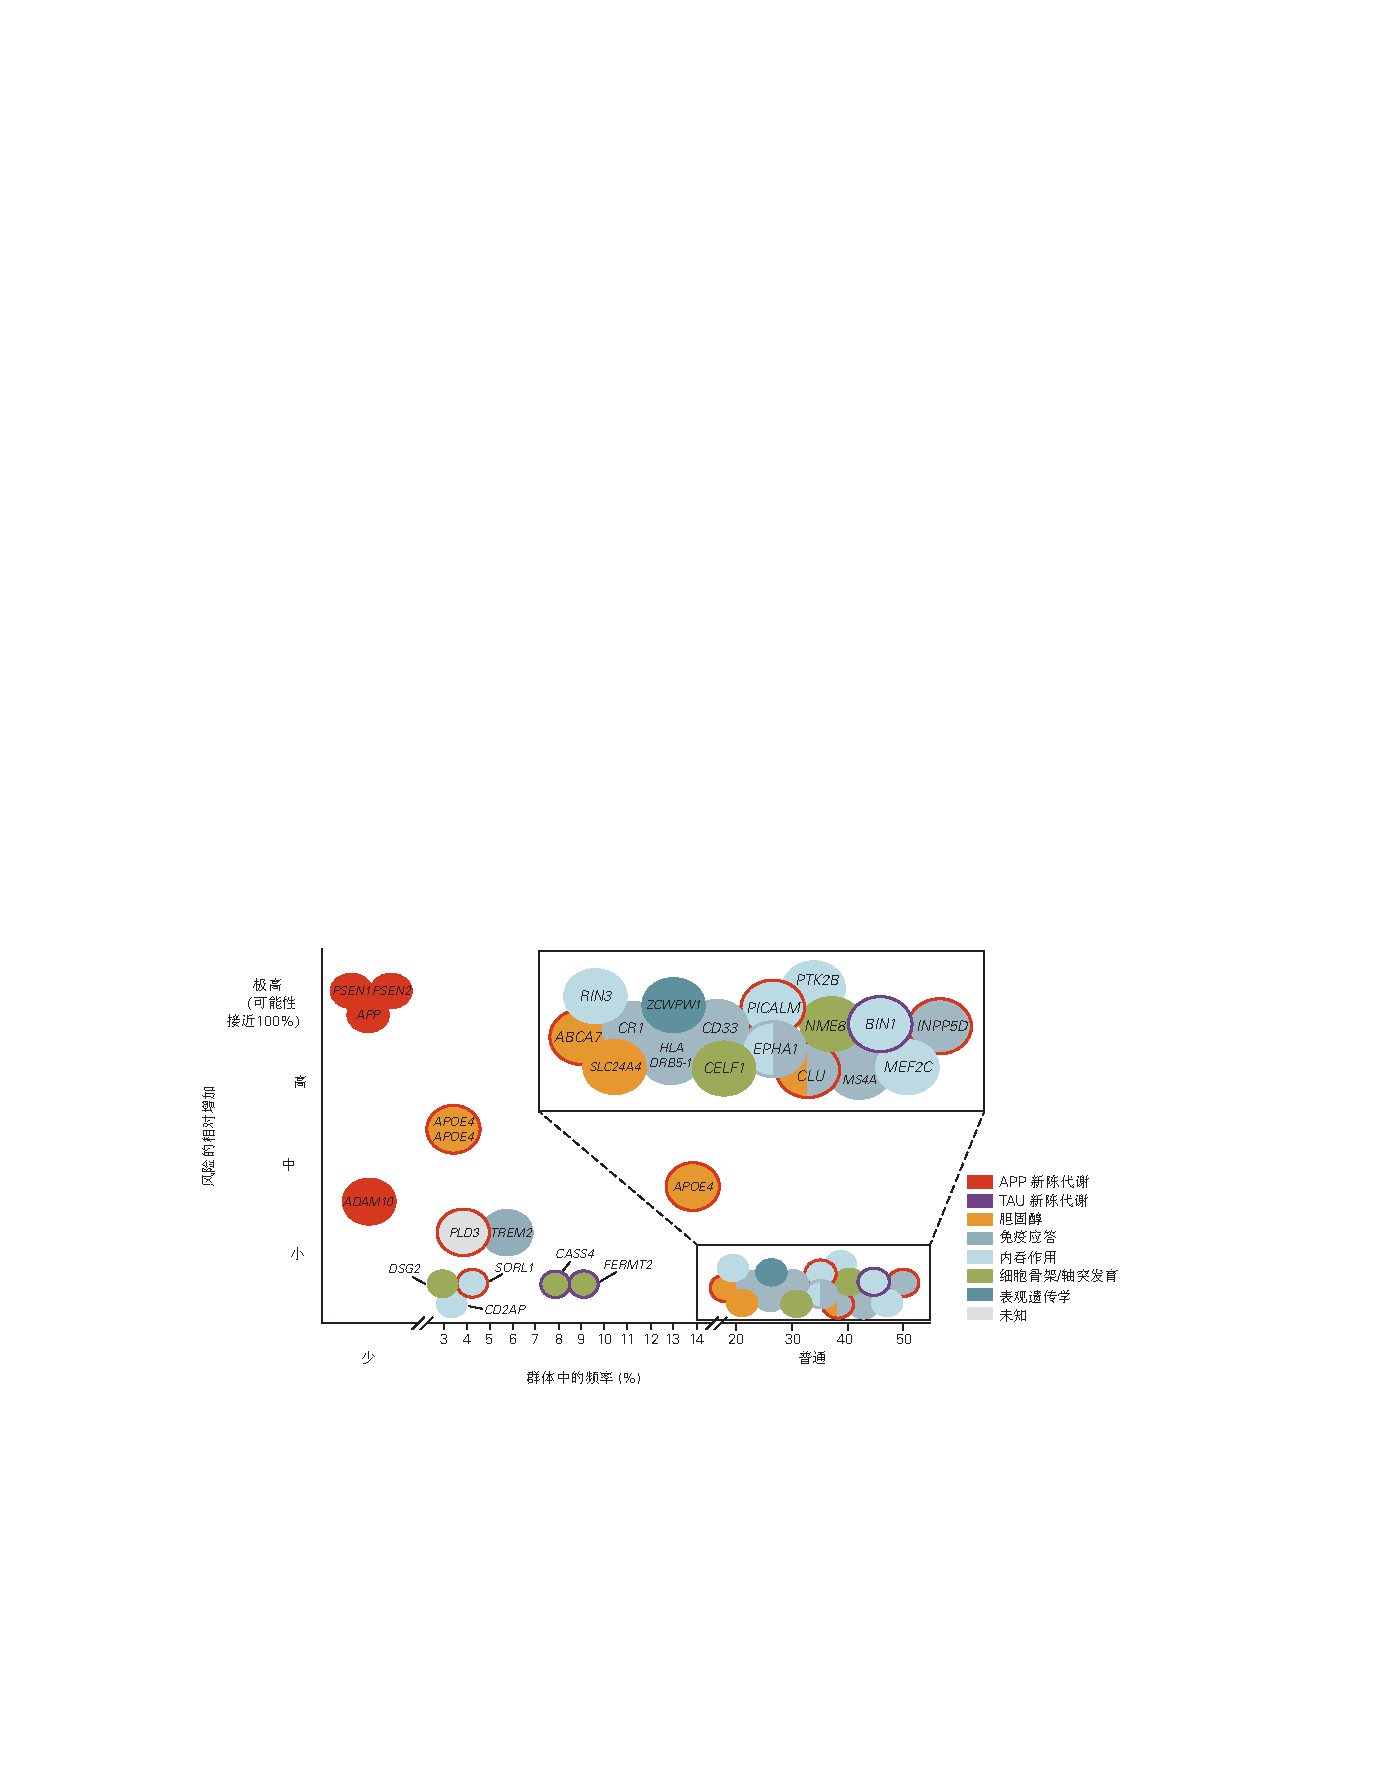
\includegraphics[width=0.9\linewidth]{chap64/fig_64_14}
	\caption{罕见和常见的基因变异导致阿尔茨海默病的风险。 数据来自\textit{全基因组关联研究}。 导致早发性家族性阿尔茨海默病(PSEN1、PSEN2 和 APP)的三个基因突变很少见,但如果他们活到中年,几乎 100\% 的携带这些突变的人都会患上阿尔茨海默病。 在人群中相对频繁出现的基因(例如 ABCA7、CLU、BIN1)周围区域或基因中发现了许多常见的遗传变化,这些变化影响阿尔茨海默病的风险,但影响程度非常小。 APOE4 是阿尔茨海默病的一种常见且强烈的遗传风险因素,存在于大约 20\% 至 25\% 的人口中(等位基因频率约为 15\%)。 相对于 APOE3 纯合子,一个 APOE4 拷贝将风险增加约 3.7 倍,两个拷贝将风险增加约 12 倍。 (经许可改编自 Karch 和 Goate 2015。)}
	\label{fig:64_14}
\end{figure}


APOE4 易患 AD 而 APOE2 预防 AD 的机制尚不确定,但 ApoE4 通过减少 Aβ 清除和促进原纤维化 (ApoE4 > ApoE3 > ApoE2) 明显促进 Aβ 聚集。
它还可能通过其他机制发挥作用,例如影响 tau、先天免疫系统、胆固醇代谢或突触可塑性,尽管这些途径仍有待研究。


许多其他基因和基因位点影响迟发性 AD 的风险。
有些是仅轻微改变风险的常见变体,而其他较罕见的变体会更大程度地增加风险(图 \ref{fig:64_14})。
例如,TREM2 基因中相对罕见的突变使 AD 的风险增加一倍或三倍,类似于具有一个 APOE4 等位基因拷贝。
这很有趣,因为 TREM2 以及另一个与 AD 风险相关的基因 CD33 仅在小胶质细胞中表达。
与其他新出现的细胞和动物模型数据一起,这一发现表明先天免疫系统参与了 AD 发病机制。
正在研究其他一些在不同程度上增加风险的罕见变异。
这些发展似乎最终会导致更加个性化的临床方法来确定 AD 的风险,特别是随着疾病治疗的出现。



\section{现在可以很好地诊断阿尔茨海默病,但可用的治疗方法并不令人满意}

在缺乏生物标志物的情况下早期诊断 AD 可能具有挑战性,因为它的初始症状可能与正常的年龄相关认知衰退或其他相关疾病的症状相似。
然而,AD 引起的轻度至中度痴呆的诊断通常相当准确。
事实上,在过去的几十年里,准确诊断疾病的能力有所提高,主要是因为三个因素。

首先,身体、神经和神经心理检查的规程变得更加复杂和标准化。
其次,增加对磁共振成像 (MRI) 揭示的结构变化的了解有助于早期诊断 AD。
例如,现在可以根据 MRI 可见的皮质变薄和心室扩大来预测哪些 MCI 患者会发展为 AD,准确率约为 80\%。
这些成像和诊断方法还有助于区分痴呆综合症,并将结构缺陷与功能缺陷联系起来。
例如,患有被称为额颞叶痴呆行为变异的疾病的患者会在早期经历人格改变,并且该阶段的 MRI 显示额叶和/或颞叶萎缩。
同样,AD 最初的困难通常集中在记忆力和注意力上,而 MRI 揭示了内侧颞叶皮层和海马体的初始改变。


第三,也许是最有前途的,淀粉样斑块和神经原纤维缠结可以通过正电子发射断层扫描 (PET) 使用强烈结合纤维状 Aβ 或聚集形式的 tau 的化合物进行可视化。
其中第一个,匹兹堡化合物 B (PIB),以高亲和力结合纤维状 Aβ;
它的放射性形式,用短寿命的碳或氟同位素标记,很容易被 PET 检测到(图\ref{fig:64_15})。
美国食品和药物管理局 (FDA) 已批准三种淀粉样蛋白显像剂:florbetapir (Amyvid)、flutemetamol (Vizamyl) 和 florbetaben (Neuraceq)。


\begin{figure}[htbp]
	\centering
	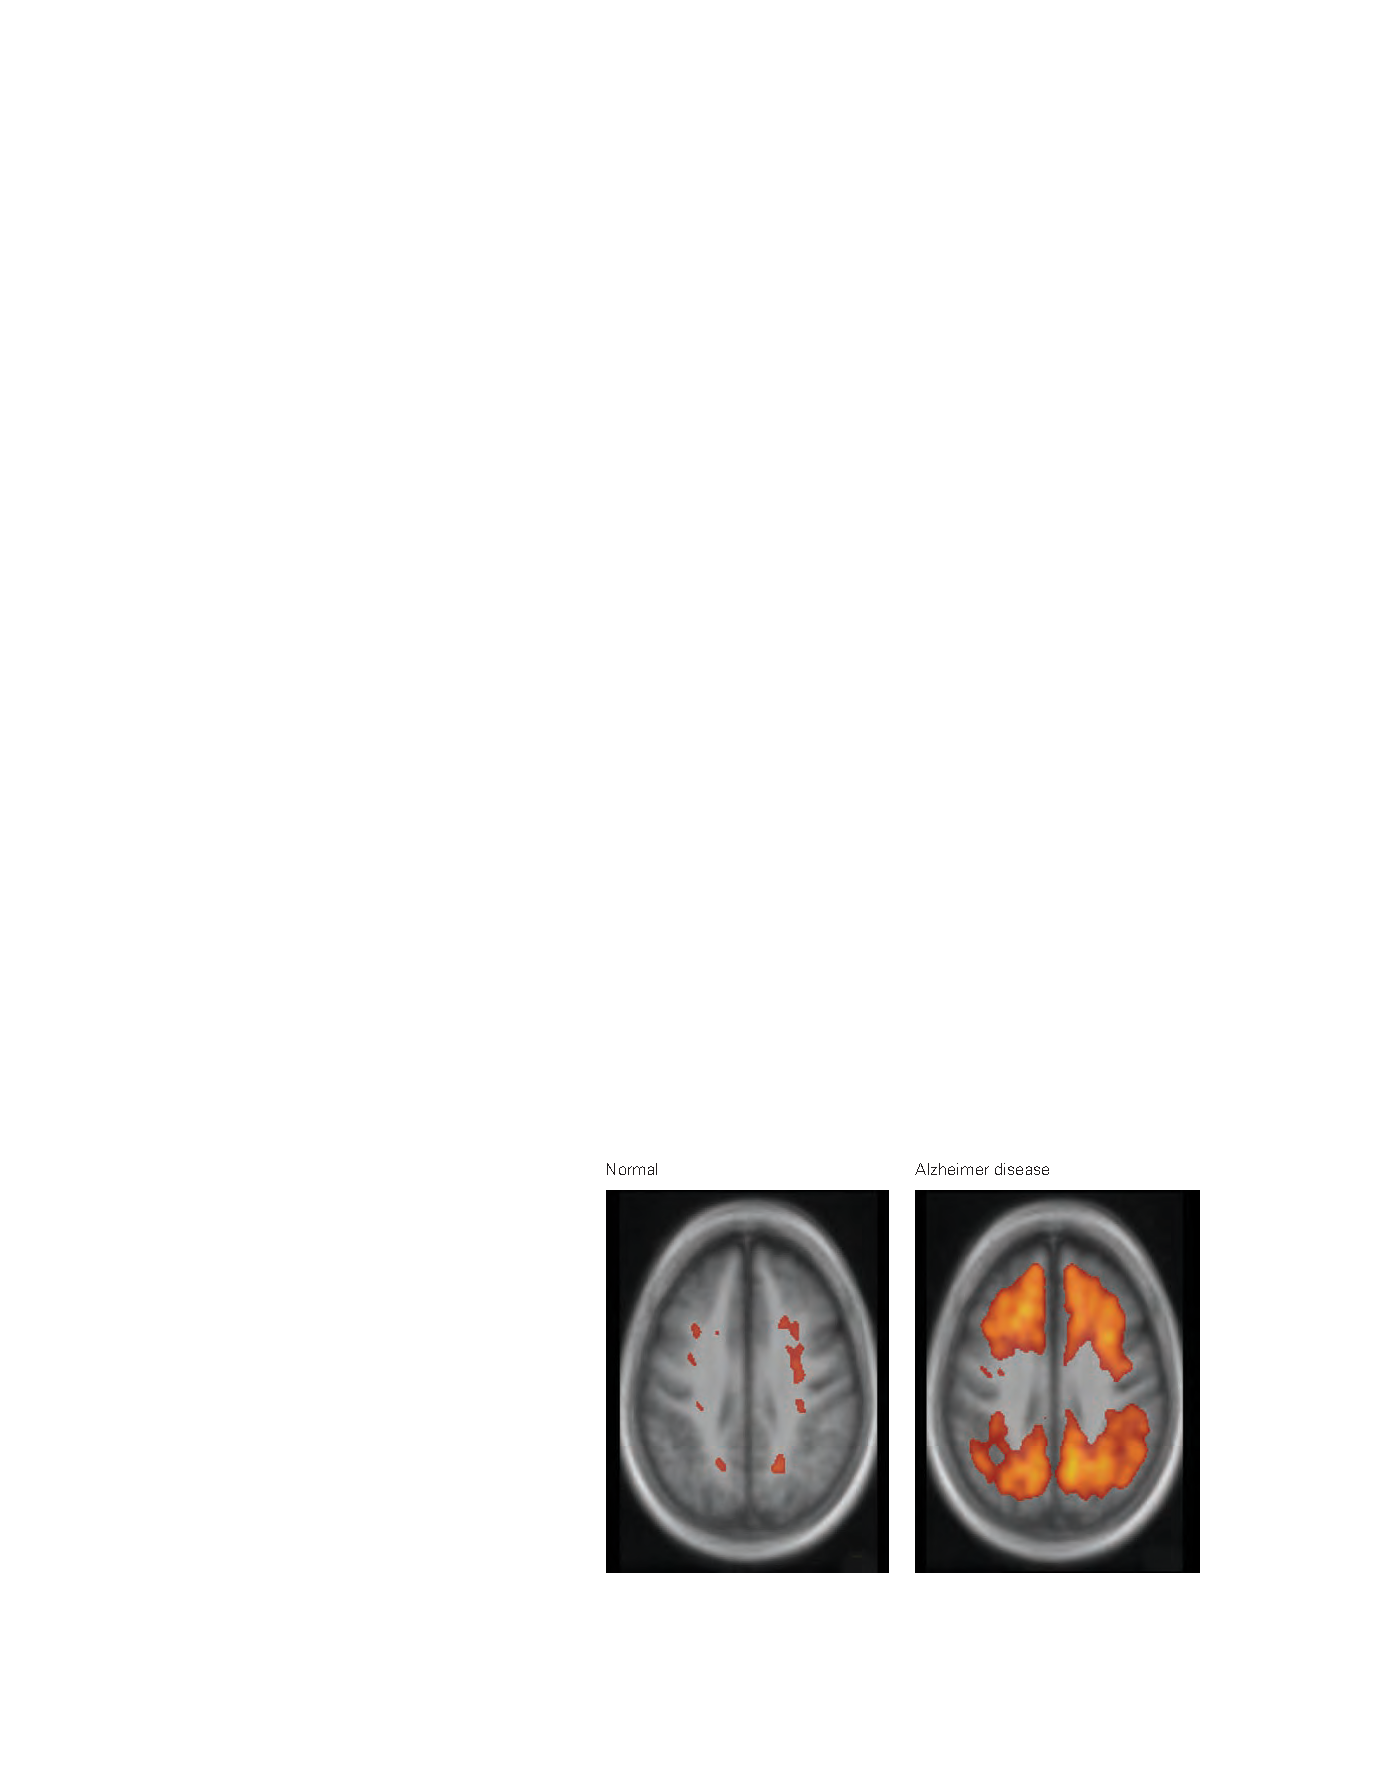
\includegraphics[width=0.6\linewidth]{chap64/fig_64_15}
	\caption{正电子发射断层扫描可以显示活体大脑中的淀粉样斑块。 Aβ 斑块的密度由这些图像中的红色区域表示,这些图像是在施用匹兹堡化合物 B (PIB) 后制作的,这是一种硫黄素 T 的荧光类似物。(图像经许可转载自 R. Buckner。)}
	\label{fig:64_15}
\end{figure}


AD 安全分子标记的可用性允许在出现临床症状之前识别疾病的早期阶段。
同样重要的是,它可以改进临床试验患者的选择,以及更敏锐地选择受试者以进行正常衰老的详细分析。
重要的是要注意,这些变化也可以在脑脊液中检测到,当存在淀粉样蛋白沉积时,Aβ42 的水平会下降,总 tau 和磷酸化形式的 tau 会随着神经变性和 tau 聚集而增加。


当然,如果有可以在早期阶段阻止或减缓其进展的可用治疗方法,改进 AD 的诊断是最有用的。
虽然我们仍然没有延迟 AD 发作或减缓 AD 进展的治疗方法,但希望我们离能够减轻症状不会太远。
虽然没有明确的证据,但有充分的证据表明各种生活方式因素可以降低患 AD 的风险。
这些包括高水平的教育、认知刺激、保持社交参与、定期锻炼、不超重以及获得适量的睡眠。
目前的疗法侧重于治疗相关症状,例如抑郁、情绪激动、睡眠障碍、幻觉和妄想。


迄今为止,主要的治疗目标之一是基底前脑中的胆碱能系统,这是一个在 AD 中受损并有助于注意力的大脑区域。
乙酰胆碱酯酶抑制剂通过抑制乙酰胆碱的分解来提高乙酰胆碱的水平,是 FDA 批准用于治疗 AD 的少数几种药物之一。
另一种药物 N-甲基-d-天门冬氨酸 (NMDA) 受体拮抗剂美金刚胺也可改善因 AD 导致的轻度至中度痴呆患者的症状。
据信美金刚的作用调节谷氨酸介导的神经传递。 然而,这些药物对认知功能和日常生活活动的影响不大。


我们对 AD 细胞生物学基础的理解的最新进展产生了几个有希望的新治疗靶点,所有这些靶点都在深入探索中。 一种方法是开发降低或调节 β- 和 γ- 分泌酶活性的药物,这些酶切割 APP 以产生 Aβ 肽和相关的可溶性细胞外和细胞内片段。
事实上,降低过表达突变 APP 的转基因小鼠中的 β- 或 γ- 分泌酶水平会减少 Aβ 沉积,并且在某些情况下会减少功能异常。


因此,制药公司开发了降低或调节人体 β- 和 γ- 分泌酶水平的药物。
这种方法的一个障碍是分泌酶还作用于 APP 以外的底物,因此降低它们的水平可能会产生有害的副作用。
对于 γ-分泌酶尤其如此,其抑制作用已导致 AD 人体试验中的毒性。
现在有几种 β-分泌酶抑制剂在 AD 的临床试验中,这些药物很可能也会进入所谓的临床前 AD 试验,此时 AD 病理正在积累但还没有认知衰退的迹象(图 64- 16)。
这种疗法的目标是延缓或预防认知能力下降和痴呆症的发生。


另一种方法是通过免疫学手段降低 Aβ 水平。
导致产生 Aβ 抗体的 Aβ 免疫和 Aβ 抗体的被动转移都已在 AD 的转基因小鼠模型中进行了测试。
两种治疗均已显示可降低 Aβ 水平、Aβ 毒性和斑块(图 \ref{fig:64_17})。
增强 Aβ 清除的机制尚不完全清楚。
血清抗体可能起到“汇”的作用,导致低分子量的 Aβ 肽从大脑中更广泛地清除到循环中,从而改变不同隔室中 Aβ 的平衡并促进 Aβ 从大脑中去除。


\begin{figure}[htbp]
	\centering
	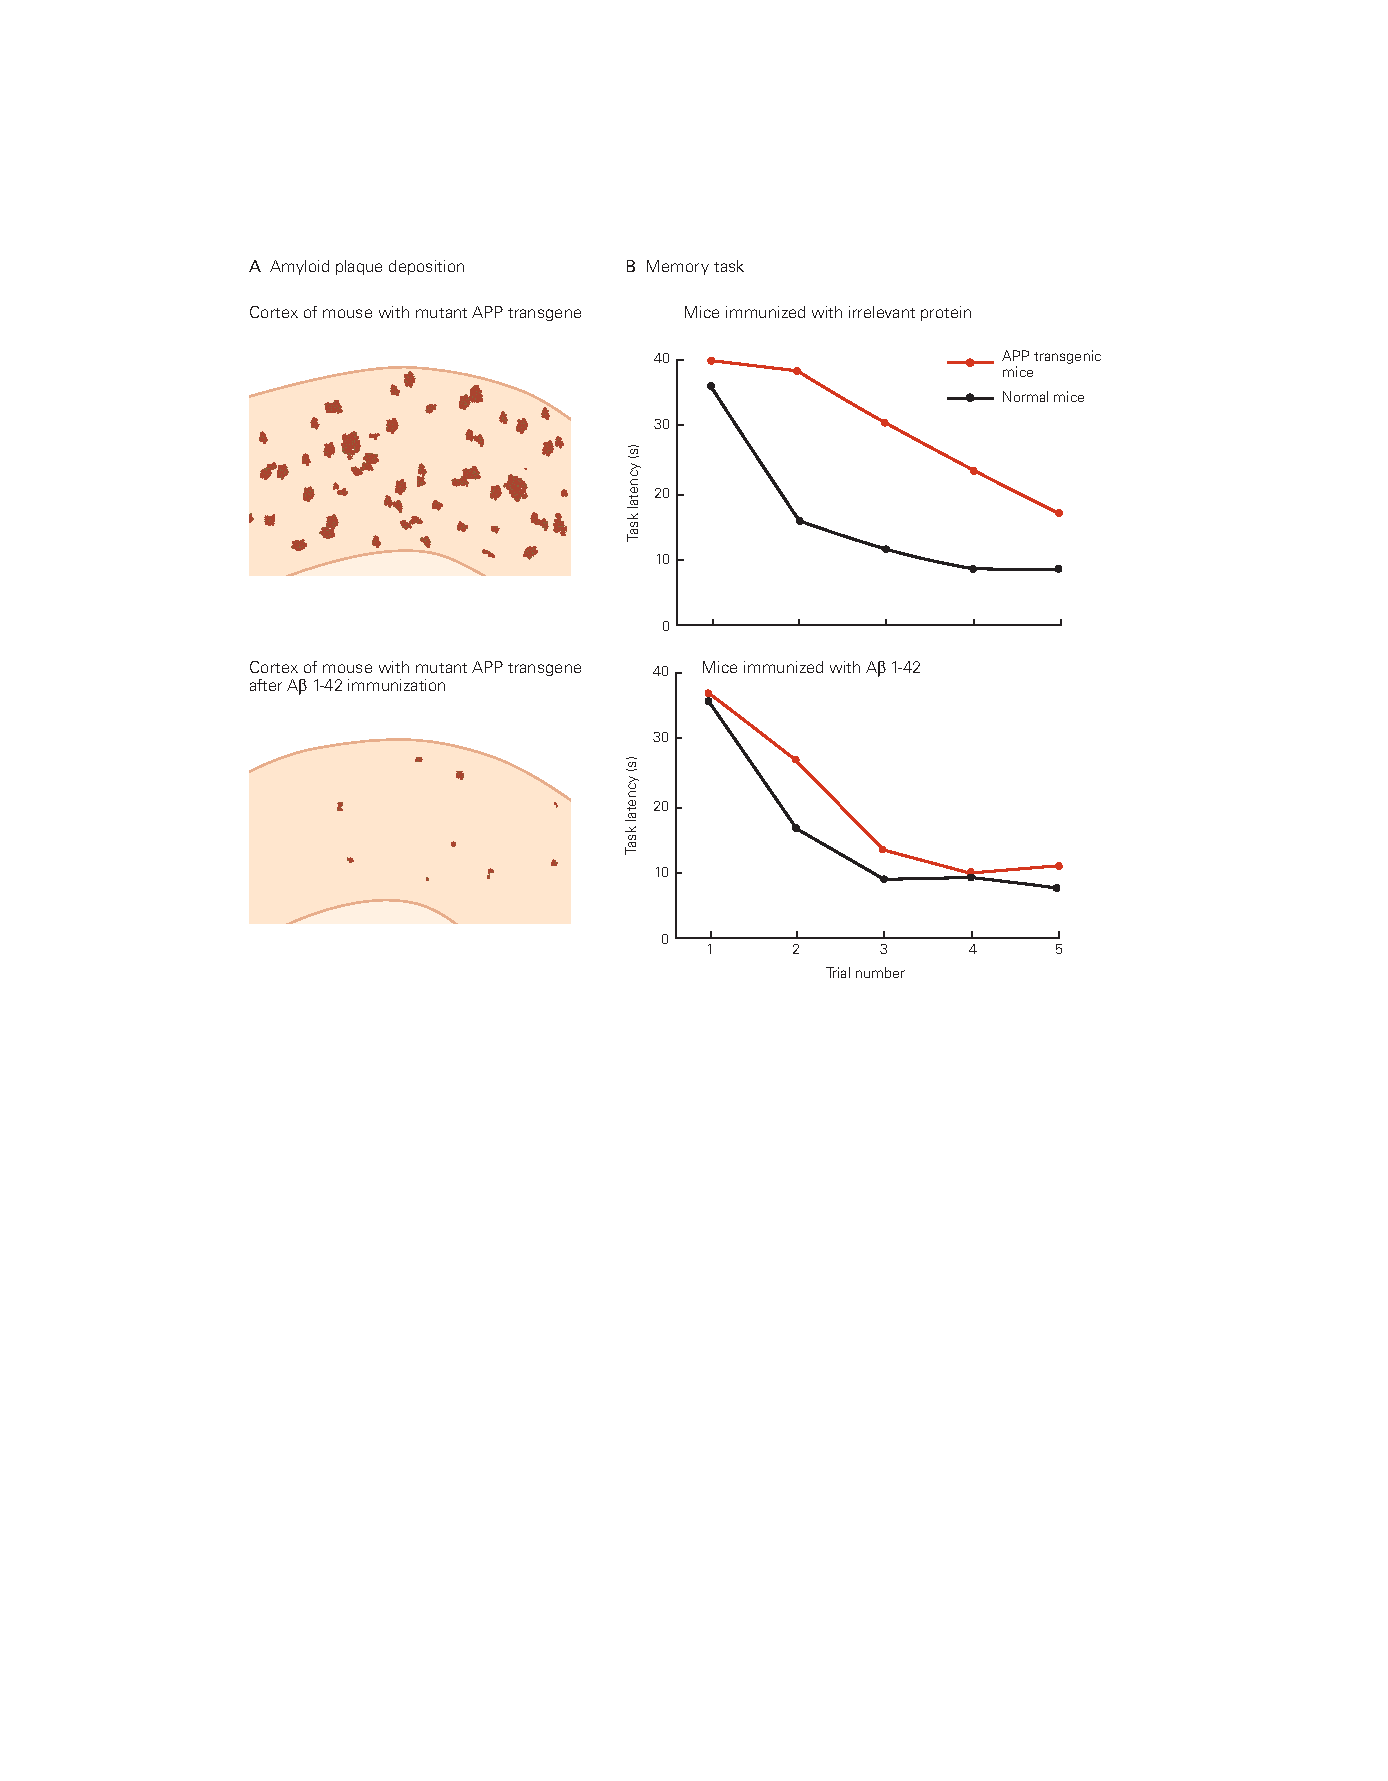
\includegraphics[width=0.8\linewidth]{chap64/fig_64_17}
	\caption{用 Aβ 肽抗体进行免疫可清除淀粉样斑块并保持表达该肽的小鼠的认知能力。 用 Aβ 肽免疫以淀粉样斑块形式形成 Aβ 沉积的小鼠。 这导致了针对 Aβ 的抗体的产生。 A. 过表达突变 APP 转基因小鼠(APP 转基因小鼠)的大脑皮层淀粉样斑块沉积的比较,该小鼠会形成淀粉样斑块。 用 Aβ 肽免疫的小鼠淀粉样斑块沉积显着减少。 (改编自 Brody 和 Holtzman 2008。)B. 两组 APP 转基因小鼠的认知表现(记忆测试)。 一组用无关蛋白免疫,另一组用 Aβ 肽免疫。 接种 Aβ 的小鼠的表现水平接近正常动物,而接种无关蛋白的小鼠则表现出严重的记忆障碍。 (经 Janus et al. 2000 许可改编。)}
	\label{fig:64_17}
\end{figure}


同样清楚的是,在大脑中,几种抗 Aβ 抗体结合可溶性或纤维状 Aβ,或两者结合。
那些与聚集形式的 Aβ 结合的物质可以刺激小胶质细胞介导的吞噬作用以去除 Aβ,尽管也有不依赖于小胶质细胞介导的吞噬作用的斑块去除。
进入大脑的可溶性 Aβ 抗体可能会降低可溶性 Aβ 的毒性。
这些发现表明,免疫治疗策略可能在 AD 患者中取得成功,特别是如果在病程中足够早地给予免疫治疗策略,在出现明显的神经元损伤和丢失之前。
在临床前和轻度 AD 中,正在进行多项针对 Aβ 的主动和被动免疫疗法的人体试验。


除了针对 Aβ,临床试验也开始针对 tau。
这是通过针对 tau 的主动和被动免疫以及在细胞培养和动物模型中可以减少 tau 聚集的小分子来完成的。
许多动物模型研究表明,某些抗 tau 抗体可以减少中枢神经系统中聚集的、过度磷酸化的 tau 蛋白的数量,并在某些情况下改善功能。
虽然 tau 主要是一种细胞质蛋白,但抗 tau 抗体可能起作用的原因之一是,如上所述,tau 聚集体可能以类似朊病毒的方式在细胞外空间中从一个细胞扩散到另一个细胞。
正是在这个空间中,抗体可能能够与 tau 相互作用并阻断这个过程。



\section{亮点}

1. 只是在过去的 50 年里,很大一部分人口才活到了 80 岁到 10 岁。
随着这种增加,神经科学家已经能够研究正常衰老以及患有与年龄相关的脑部疾病的个体的大脑变化。


2. 随着年龄的增长,各种大脑功能会发生微妙的变化,包括处理速度和记忆存储的下降以及睡眠的变化。
这些变化的根本原因可能是脑萎缩和白质完整性丧失。
然而,总的来说,神经元数量并没有显着减少,这可以解释正常衰老时发生的大脑功能变化。


3. 正常衰老过程中发生的认知变化不会致残。
当记忆力和认知功能的其他领域随着年龄的增长而下降超过预期,以至于其他人会注意到并轻度影响一个人的日常生活时,这种综合症称为轻度认知障碍 (MCI)。


4. MCI 不是一种疾病,它是一种综合症。 大约 50\% 的 MCI 患者将阿尔茨海默病 (AD) 作为 MCI 的根本原因。
其他可能导致 MCI 的情况包括抑郁症、脑血管疾病、路易体病、代谢紊乱,以及针对其他疾病开出的会引起中枢神经系统副作用的药物。


5. AD 是痴呆症最常见的原因,表现为记忆力和其他足以损害社会和职业功能的认知能力的丧失。
在美国,AD 约占痴呆病例的 70\%,其余主要由脑血管疾病、帕金森和路易体痴呆以及额颞叶痴呆引起。


6. AD 的病理学特征是两种蛋白质 Aβ 肽和 tau 的聚集形式在大脑中的积累。
Aβ 以纤维状形式积聚在脑实质和小动脉壁(称为脑淀粉样血管病)中的称为淀粉样斑块的细胞外结构中。
Tau 在细胞体和树突中的神经原纤维缠结中积累。


7.除了阿尔茨海默病大脑中蛋白质聚集体的积累,随着疾病的进展,还会出现明显的脑萎缩以及突触和神经元丢失。
还有强烈的神经炎症反应,尤其是在涉及小胶质细胞和星形胶质细胞的淀粉样斑块周围。


8. AD 的病理学开始于认知衰退或疾病的 MCI 阶段开始前约 15 年。
新皮质中的 Aβ 积聚似乎以明显异常的水平引发疾病,随后 tau 聚集体从内侧颞叶扩散到新皮质的其他区域。
症状出现之前的阿尔茨海默病病理学阶段称为临床前 AD。


9. 重要数据表明,Aβ 肽的某些聚集形式会导致阿尔茨海默病大脑中的突触和神经元损伤,但与认知能力下降更好相关的是 tau 蛋白聚集形式的存在和积累。


10. AD 有两种主要形式。
第一种是显性遗传性 AD,占阿尔茨海默病患者的比例不到 1\%,是由编码蛋白质 APP、PS1 和 PS2 的三个基因之一的突变引起的;
这种形式导致临床疾病在 30 到 50 岁之间发作。遗传、生物化学和其他研究表明,导致常染色体显性 AD 的基因通过 Aβ 肽在大脑中的早期积累来实现。
第二种形式,迟发性AD,发病年龄为65岁或更晚,占病例的99\%以上。
虽然年龄是迟发性 AD 的最大危险因素,但遗传因素也有影响。 APOE 基因是迄今为止 AD 的最大遗传因素,APOE4 变体增加风险,APOE2 变体降低风险。
影响风险的其他基因中还有许多其他常见的遗传变异。
其他基因(如 TREM2)中也存在罕见变异,这些变异将风险增加到与 APOE4 一个拷贝相关的水平。
尽管如此,普遍认为散发性和家族性 AD 发病机制的主要特征相似。


11. 除了 AD 的临床症状和体征外,淀粉样蛋白和 tau 成像以及脑脊液标记物可以确定活人是否存在认知衰退的阿尔茨海默病症。


12. 目前只有 AD 的对症疗法充其量只能带来适度的益处。
许多影响 Aβ 或 tau 的产生、清除和聚集的潜在疾病缓解疗法正在人体中进行测试。
尽管这些疗法尚未获得批准,但希望在未来几年内,其中一种或多种疗法将开始显示出明显的益处。


